%ACTIVATE BOTH FOR SVG WITH ANIMATIONS
\RequirePackage[dvips]{xcolor}
\documentclass[dvisvgm,11pt,aspectratio=169]{beamer}
%\documentclass[11pt,aspectratio=169]{beamer}
\usepackage[utf8]{inputenc} 
\usepackage[spanish,es-tabla]{babel}
\decimalpoint
\usepackage{amsmath}
\usepackage{amsfonts}
\usepackage{amssymb}
\usepackage{bm}
\usepackage{xcolor,colortbl}
\usepackage{textcomp}
\usepackage{amssymb}
\usepackage{tikz}
\usepackage[export]{adjustbox}
\usepackage{url}
\usepackage{graphicx}
\usepackage{pdfrender}
\usepackage{float}
\usepackage{longtable}
\usepackage{appendixnumberbeamer}
%\usepackage{chemmacros}
\usepackage{braket}
\usepackage{multirow}
\usepackage{booktabs}
\usepackage{color, colortbl}
\usepackage{subcaption}
\usepackage[dvisvgm]{animate}
\usepackage{empheq}
\usepackage{setspace}


\usepackage{tikz}
\usepackage{pgfcalendar}
\usepackage{pgfgantt}

\usepackage[sfdefault]{FiraSans}

\usefonttheme[onlymath]{serif}
\usetikzlibrary{shapes.geometric,arrows,calc}

%%%%%%%%%%%%%%%%%%%%%%%%%%%%%%%%%%%%%%%%%%%%%%%%%%%%%%%%%%%%%%%%%%%%%%%%%%%%%%%
% PageDown, PageUp key event handling; navigation symbols
%%%%%%%%%%%%%%%%%%%%%%%%%%%%%%%%%%%%%%%%%%%%%%%%%%%%%%%%%%%%%%%%%%%%%%%%%%%%%%%
\usepackage[totpages]{zref}
\usepackage{atbegshi}
\usepackage{fontawesome}
\setbeamertemplate{navigation symbols}{}
\AtBeginShipout{%
  \AtBeginShipoutAddToBox{%
    \special{dvisvgm:raw
      <defs>
      <script type="text/javascript">
      <![CDATA[
        document.addEventListener('keydown', function(e){
          if(e.key=='PageDown'){
            \ifnum\thepage<\ztotpages
              document.location.replace('\jobname-\the\numexpr\thepage+1\relax.svg');%
            \fi
          }else if(e.key=='PageUp'){
            \ifnum\thepage>1
              document.location.replace('\jobname-\the\numexpr\thepage-1\relax.svg');%
            \fi%
          }
        });
      ]]>
      </script>
      </defs>
    }%
  }%
  \AtBeginShipoutUpperLeftForeground{%
    \raisebox{-\dimexpr\height+0.5ex\relax}[10pt][0pt]{\makebox[\paperwidth][r]{%
      \footnotesize\color{structure!40!}%
      \ifnum\thepage>1%
        \href{\jobname-\the\numexpr\thepage-1\relax.svg}{\faArrowLeft}%
      \else%  
        \textcolor{lightgray}{\faArrowLeft}%  
      \fi\hspace{0.5ex}%
      \ifnum\thepage<\ztotpages%
        \href{\jobname-\the\numexpr\thepage+1\relax.svg}{\faArrowRight}%
      \else%
        \textcolor{lightgray}{\faArrowRight}%  
      \fi%
      \hspace{0.5ex}%
    }}%
  }%  
}%
%%%%%%%%%%%%%%%%%%%%%%%%%%%%%%%%%%%%%%%%%%%%%%%%%%%%%%%%%%%%%%%%%%%%%%%%%%%%%%%



%%%%%%%%%%%%%%%%%%%%%%%%%%%%%%%%%%%%%%%%%%%
%Para los diagramas de flujo
%%%%%%%%%%%%%%%%%%%%%%%%%%%%%%%%%%%%%%%%%%%

\tikzstyle{startstop} = [rectangle,text=white, rounded corners, minimum width=3cm, minimum height=1cm,text centered, draw=black, fill=nuno]
\tikzstyle{io} = [trapezium, trapezium left angle=70, trapezium right angle=110, minimum width=3cm, minimum height=1cm, text centered, draw=black, fill=blue!30]
\tikzstyle{process} = [rectangle, minimum width=3cm, minimum height=1cm, text centered, draw=black, fill=ndos]
\tikzstyle{decision} = [diamond, aspect=2, minimum width=3cm, minimum height=1cm, text centered,text width=3cm, draw=black, fill=ntres]
\tikzstyle{arrow} = [thick,->,>=stealth]
%
\makeatletter
\let\beamer@writeslidentry@miniframeson=\beamer@writeslidentry
\def\beamer@writeslidentry@miniframesoff{%
  \expandafter\beamer@ifempty\expandafter{\beamer@framestartpage}{}% does not happen normally
  {%else
    % removed \addtocontents commands
    \clearpage\beamer@notesactions%
  }
}
\newcommand*{\miniframeson}{\let\beamer@writeslidentry=\beamer@writeslidentry@miniframeson}
\newcommand*{\miniframesoff}{\let\beamer@writeslidentry=\beamer@writeslidentry@miniframesoff}
\makeatother

\definecolor{Gray}{gray}{0.85}
\definecolor{muno}{HTML}{63595c}
\definecolor{mdos}{HTML}{646881}
\definecolor{mtres}{HTML}{5ad2f4}
\definecolor{nuno}{HTML}{33658a}
\definecolor{ndos}{HTML}{86bbd8}
\definecolor{ntres}{HTML}{f6ae2d}
\definecolor{test1}{HTML}{1f271b}
\definecolor{test2}{HTML}{eff2c0}
\definecolor{test3}{HTML}{0b4f6c}
\definecolor{test4}{HTML}{306b34}

\newcolumntype{a}{>{\columncolor{cyan}}c}
\newcolumntype{b}{>{\columncolor{Gray}}c}


\usepackage[backend=biber,style=chem-acs,citestyle=verbose]{biblatex}
\bibliography{library}

\newcommand{\pvec}[1]{\vec{#1}\mkern2mu\vphantom{#1}}

\newcommand\TBox[2][]{%
  \tikz\node[draw,ultra thick,align=center,#1] {#2};\hskip2pt}

\usetheme[sectionpage=progressbar,numbering=fraction,progressbar=frametitle,block=fill]{metropolis}    % Use metropolis theme

\setbeamercolor{normal text}{fg=test1,bg=white}
\setbeamercolor{progress bar}{fg=test3,bg=test2}

\definecolor{light-gray}{gray}{0.89}


\makeatletter
\setlength{\metropolis@frametitle@padding}{1.8ex}% <- default 2.2 ex
\setbeamertemplate{frametitle}{%
    \nointerlineskip%
    \begin{beamercolorbox}[%
        wd=\paperwidth,%
        sep=0pt,%
        leftskip=\metropolis@frametitle@padding,%
        rightskip=\metropolis@frametitle@padding,%
        ]{frametitle}%
        \metropolis@frametitlestrut@start%
        \insertframetitle%
        \nolinebreak%
        \metropolis@frametitlestrut@end%
        \hfill
        \hyperlink{contents}{
\includegraphics[height=3ex,keepaspectratio,valign=c]{img/uaml}}
    \end{beamercolorbox}
    \usebeamertemplate*{progress bar in head/foot}
}

\setlength{\metropolis@progressinheadfoot@linewidth}{2pt}

\setbeamertemplate{sidebar right}{}
\setbeamertemplate{background}{\tikz[overlay,remember picture]\node[opacity=0.08]at (11,-6){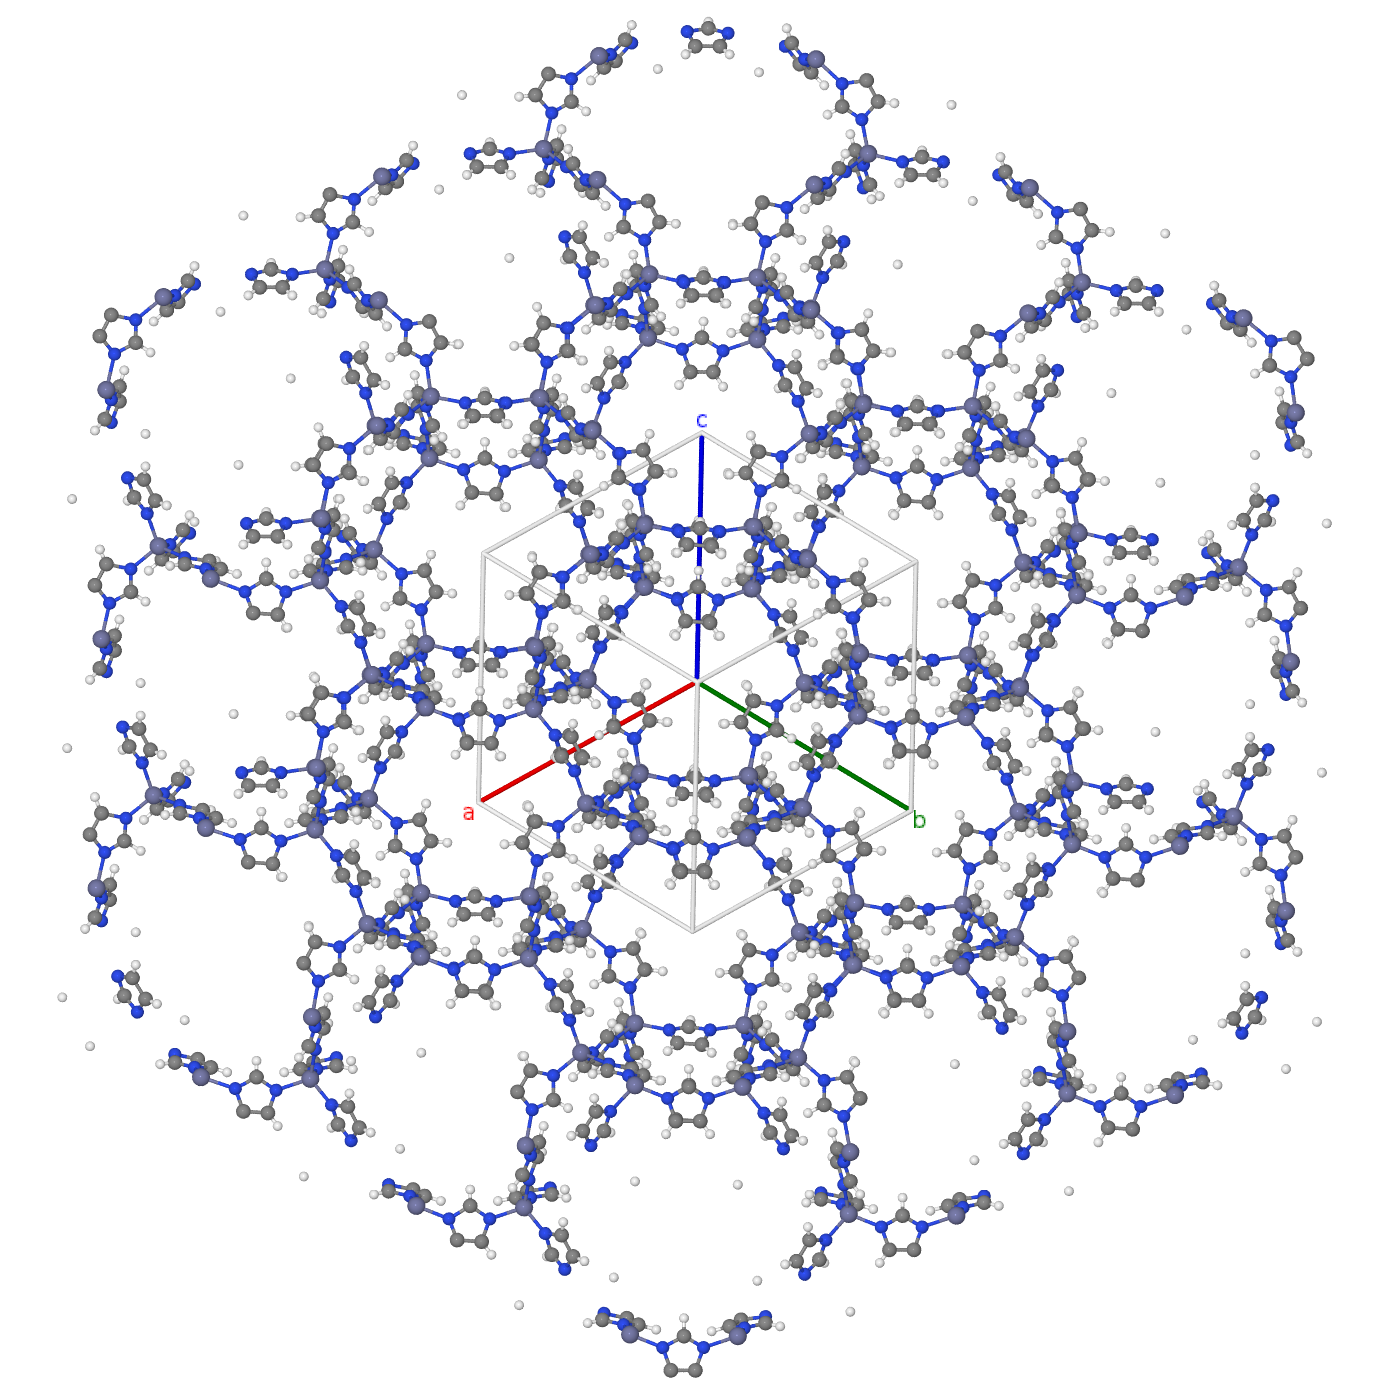
\includegraphics[width=10cm]{img/zif8}};}


\setbeamertemplate{title page}{%
\begin{tikzpicture}[remember picture,overlay]
\fill[test1]
  (current page.north west) rectangle (current page.south);
\node[anchor=east] 
  at ([yshift=0.3cm]current page.east) (author)
  {\parbox[t]{.6\paperwidth}{\raggedleft%
    \usebeamerfont{author}\textcolor{test1}{%
    \insertauthor}}};
\node[anchor=south] 
  at ([xshift=-1.5cm,yshift=0.3cm]current page.south) (institute)
  {\parbox[t]{.30\paperwidth}{\raggedright%
    \usebeamerfont{institute}\textcolor{white}{\insertinstitute}}};
\node[anchor=south west] 
  at ([yshift=0pt]current page.south west) (logo)
  {\parbox[t]{.19\paperwidth}{\raggedleft%
    \usebeamercolor[fg]{titlegraphic}\inserttitlegraphic}};
\node[anchor=north east]
  at ([yshift=0pt,xshift=0pt]current page.north east) (title)
  {\setstretch{1.5}\parbox[t]{0.5\textwidth}{ \raggedleft%
 \usebeamerfont{author}\textcolor{test1}{%
    \Large  \firamedium{\inserttitle}}}};	
 \node[anchor=west]
  at ([yshift=0.6cm,xshift=-0.2cm]current page.west) (img1)
  {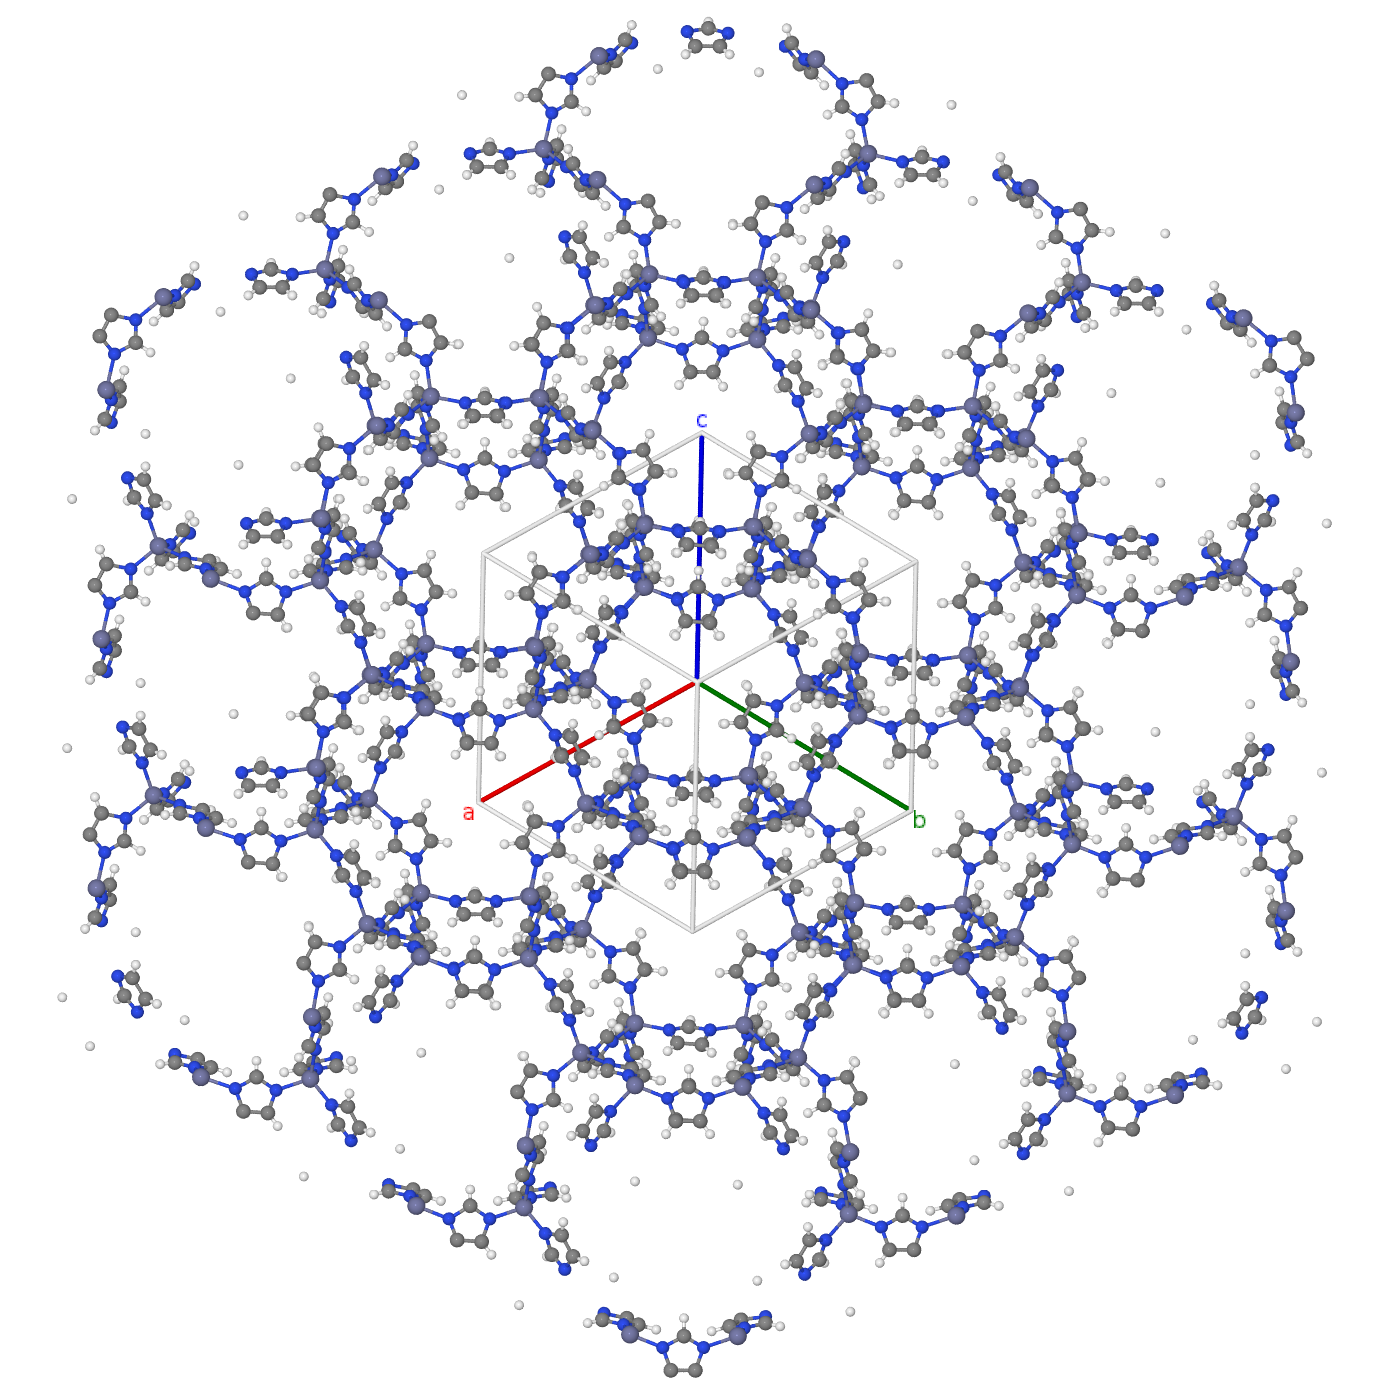
\includegraphics[width=8cm]{img/zif8}};
  \node[anchor=south east]
  at ([yshift=0.7cm,xshift=-1.9cm]current page.south east) (img2)
  {\Large $\langle \mu^\mathbf{0} \nu^\mathbf{g}|\sigma^\mathbf{h} \omega^{\mathbf{h+g'}} \rangle$};
  \node[anchor=south east]
  at ([yshift=0.1cm,xshift=-1.9cm]current page.south east) (img2)
  {\footnotesize Ciudad de México, Junio 2021};
  \node[anchor=south east]
  at ([yshift=1.4cm,xshift=-2.5cm]current page.south east) (img3)
  {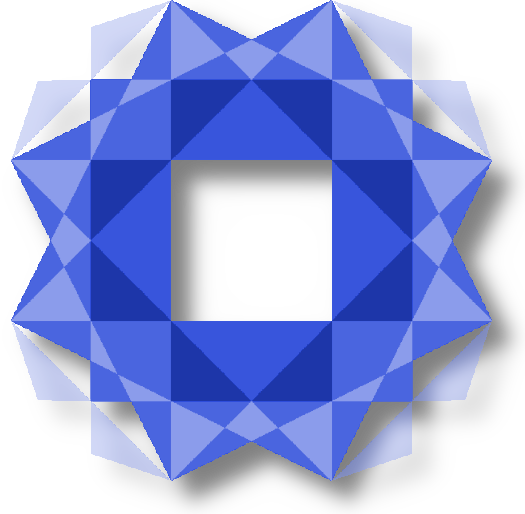
\includegraphics[width=2cm]{img/bz1}};
    \node[anchor=east]
  at ([yshift=-60pt,xshift=-20pt]current page.east) (subtitle)
  {\parbox[t]{.6\paperwidth}{\raggedleft\usebeamerfont{subtitle}\textcolor{black}{\insertsubtitle}}};
\end{tikzpicture}
}

\setbeamerfont{note}{size=\tiny}

\setbeamertemplate{section in toc}[ball unnumbered]

\title{Evaluación de integrales bielectrónicas en sistemas periódicos usando cómputo heterogéneo}
\date{Junio 2021}
\author{\textit{Trabajo de Investigación II}\\\textit{Alumno:} \firamedium{Marcos Rivera Almazo} \\ \textit{\firabook Asesor:} \firamedium{Dr. Jorge Garza Olguín}}
\institute{Departamento de Química\\Área de Fisicoquímica Teórica}
\titlegraphic{
\includegraphics[width=3.5cm]{img/uam3}}

% \setbeamertemplate{footnote}{
%        {\insertfootnotemark}
%        \parbox[b][2cm]{2cm}{
%            \insertfootnotetext%
%        }%
%    }
%\addtobeamertemplate{footnote}{}{}
\setbeamertemplate{footline}{%
  \begin{beamercolorbox}[wd=\textwidth, sep=1.5ex,ht=0.7ex]{footline}% <- default 3ex
  	\tiny
    \usebeamerfont{page number in head/foot}%
    \usebeamertemplate*{frame footer}
    \hfill%
    \usebeamertemplate*{frame numbering}
  \end{beamercolorbox}%
}
\makeatother
\makeatletter
% Alternative A: footnote rule
%\renewcommand*{\footnoterule}{\kern -3pt \hrule \@width 2in \kern 8.6pt}
% Alternative B: no footnote rule
% \renewcommand*{\footnoterule}{\kern 6pt}
\renewcommand{\footnotesize}{\tiny}
\makeatother


\begin{document}
%%%%%%%%%%%%%%%%%%%%%%%START%%%%%%%%%%%%%%%%%%%%%%%%%%%%%%%%%%%%%%%%
 
  \begin{frame}  
  \date{Noviembre 2020}
  \titlepage
  \end{frame}

  \begin{frame}{Contenido}
  \tikz [remember picture,overlay]
    	\node at
        	([yshift=3.3cm,xshift=-3.7cm]current page.south east) 
        	%or: (current page.center)
        	{
\includegraphics[width=7.5cm]{img/muraledit}};
  \hypertarget{contents}{}
  \tableofcontents
  \end{frame}


\section{Introducción}
%\subsection{Resumen}
\begin{frame}{Resumen}

	\begin{block}{Objetivo principal}
	Elaborar una biblioteca para la evaluación de integrales bielectrónicas (IB) en sistemas periódicos usando cómputo heterogéneo.
	\end{block}

	\begin{block}{Objetivos particulares}
		\begin{itemize}
			\item \textbf{Implementar una rutina de clasificación para seleccionar las integrales que deben ser resueltas.}
			\item Acoplar a una rutina que resuelva las integrales seleccionadas.
			\item Integrar directivas sencillas para la ejecución con cómputo heterogéneo.
			%\item Optimizar la biblioteca resultante para mejorar el tiempo de ejecución.
		\end{itemize}
	\end{block}
\end{frame}

\begin{frame}
\begin{columns}
\begin{column}{0.8\textwidth}
	La biblioteca debe cumplir con:
	\begin{itemize}
		\item Sencilla de integrar.
		\item Lógica del programa accesible a terceros. 
		\item Documentación extensiva para su desarrollo futuro.
		\item Algoritmos eficientes en CPU y GPU.
	\end{itemize}
	Se utilizará:
	\begin{itemize}
		\item Lenguaje C++17 y modelo Orientado a Objetos.
		\item OpenACC para la ejecución en GPU.\footnotemark  SYCL como alternativa.\footnotemark
		\item Evaluar las IB usando rutinas de un tercero.
		\item Tomar como referencia la metodología usada en Crystal.\footnotemark
	\end{itemize}
	
	\footcitetext{OpenACC2019}
	\footcitetext{SYCL2019}
	\footcitetext{Demichelis2008}
	\end{column}
	\begin{column}{0.2\textwidth}
	\centering
	
	
\includegraphics[width=0.6\textwidth]{img/cpp}	\\
	\vspace{1cm}		
	
\includegraphics[width=0.98\textwidth]{img/openacc}\\
	\vspace{1cm}
	
\includegraphics[width=0.98\textwidth]{img/cry}

	\end{column}
\end{columns}
\end{frame}



\begin{frame}{Avances previos}
\begin{minipage}{0.98\textwidth}

	\begin{itemize}
		\item Clase \textit{Crystal}:
		\begin{itemize}
			\item Lectura y almacenamiento de la información básica (parámetros de celda, coordenadas atómicas, funciones de base).
			\item Conversión de ésta de coordenadas relativas a cartesianas.
			\item Funciones para consultar la información.
		\end{itemize}
		\item Artículo de las interacciones de un MOF con CO y SO$_2$.\footnotemark
	\end{itemize}
	\centering
	
\includegraphics[width=0.6\textwidth]{img/Rivera2021}
	\footcitetext{Rivera-Almazo2021}
	
\end{minipage}
\end{frame}

\section{Avances del periodo}
\begin{frame}{Estado general del código}
	Propuesta actual de diseño:
	\begin{itemize}
		\item Clase \textit{Crystal}: Almacenado de la información geométrica y de la base.
		\item Clase \textit{Preclas}: Preprocesamiento de la información de entrada.
		\item Clase \textit{CryBiInfo}: Coordinación del proceso de cálculo.
		\item Clases \textit{CryCol} y \textit{CryEx}: Matrices Coulómbica y de Intercambio.
	\end{itemize}
\end{frame}

\begin{frame}{Secciones de código producidas}
	\textit{Preclas}:
			\begin{itemize}
				\item *Producción, almacenado y ordenamiento de puntos de la malla en espacio real, dentro de un cubo circunscrito a una esfera.
				\item Análisis de funciones de base y obtención de la información de Gaussianas Adjuntas (GA) por átomo y capa.
				\item *Lista de pares atómicos dado un filtrado por GAs.
				\item Lista de pares de capas dado un filtrado por GAs y el filtrado atómico.
				\item Funciones para consultar la información.
			\end{itemize}
\end{frame}

\begin{frame}{Secciones de código producidas (cont.)}
	Herramientas de uso general:
		\begin{itemize}
			\item Funciones para calcular $ln$ del traslape entre gaussianas tipo s.
			\begin{itemize}
				\item Dados los exponentes y las coordenadas $\mathbf{R_a, R_b}$ y $\mathbf{g}$.
				\item Dados los exponentes y la distancia $R_{ab}$
			\end{itemize}
			\item Función para transformar vectores en coordenadas relativas a cartesianas.
			\item Función para calcular el módulo de un vector a partir de sus coordenadas relativas.
		\end{itemize}
\end{frame}

\begin{frame}{Sistemas de prueba}
\begin{columns}
\begin{column}{0.7\textwidth}
	Para probar la correcta ejecución del programa se utilizan los siguientes sistemas:
	\begin{itemize}
		\item Cuarzo-$\alpha$ (SiO$_2$). Celda trigonal.$^\diamondsuit$
		\item FeN$_4$. Celda triclínica.
		\item Ilmenita (CaSnO$_3$). Celda trigonal.
		\item Helio. Celda hexagonal.*
		\item MOF NOTT-401, Celda tetragonal.*
		\item SiO$_2$. Celda tetragonal.*
	\end{itemize}
	($^\diamondsuit$ Usado en la documentación de Crystal.)
	
	(*Sistemas previamente estudiados.)
\end{column}
\begin{column}{0.3\textwidth}
\centering
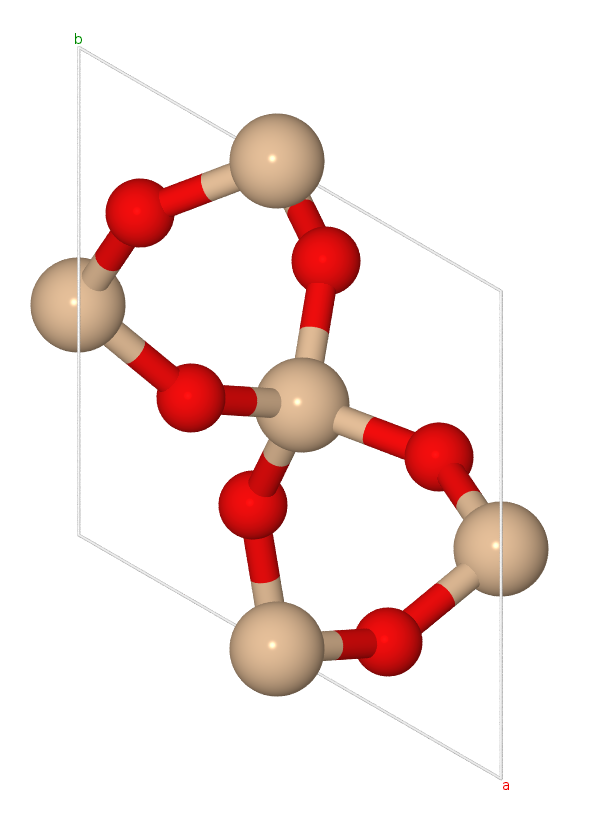
\includegraphics[width=0.4\textwidth]{img/quartz}
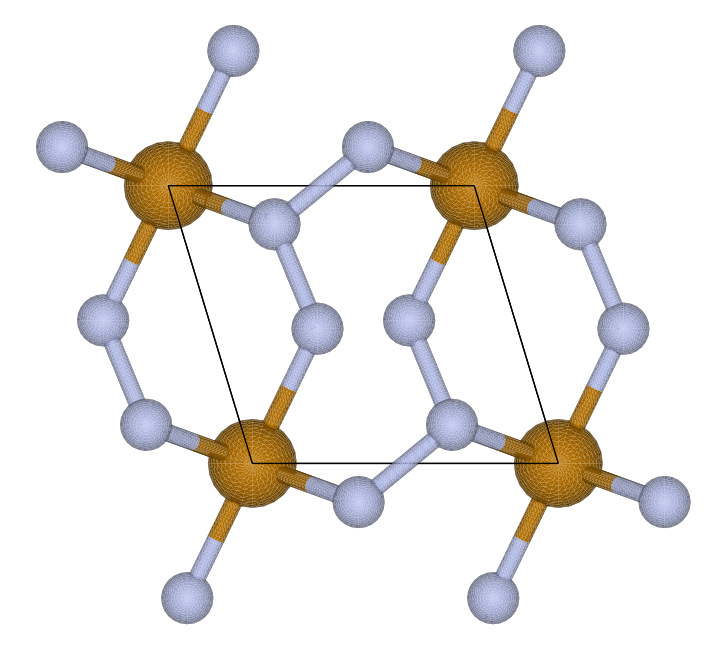
\includegraphics[width=0.5\textwidth]{img/FeN4}
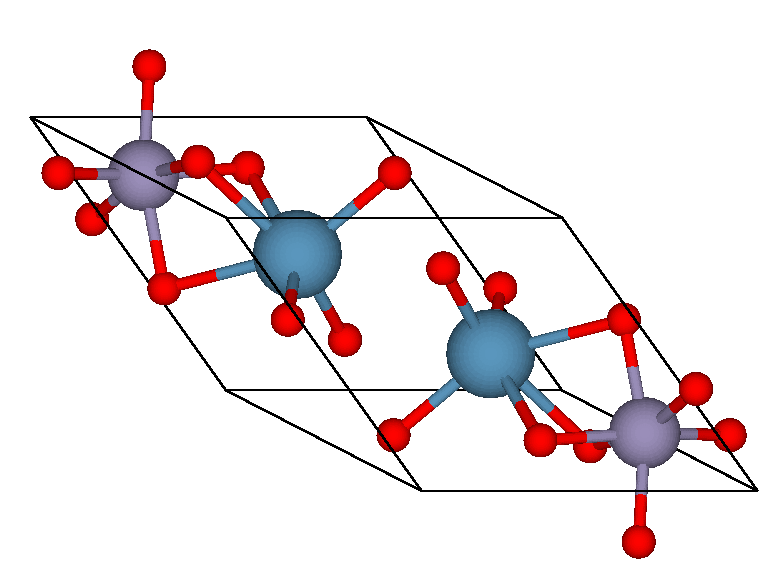
\includegraphics[width=0.7\textwidth]{img/ilmenite}
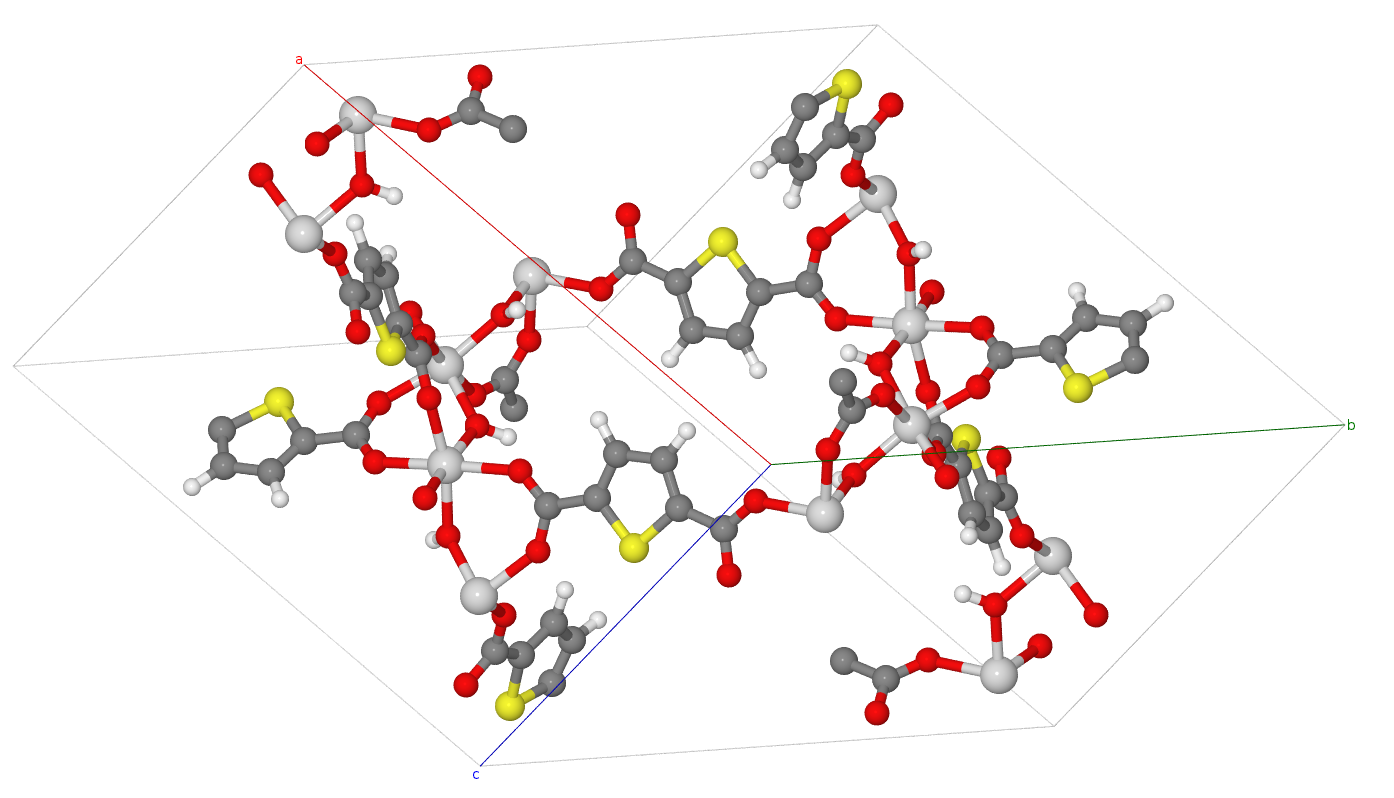
\includegraphics[width=0.9\textwidth]{img/nott401}

\end{column}
\end{columns}

\end{frame}

\section{Desarrollo del código}
\begin{frame}{Criterio de traslape de GAs}
	Siguiendo el procedimiento usado en Crystal, filtraremos pares de átomos y capas dado el traslape de GAs, \textbf{gaussianas tipo s cuyo exponente es el menor asignado al átomo/capa.} 
	El traslape entre dos GAs está dado por: 
	\begin{equation}\label{rab}
    \rho_{ab} = \int d\tau g_a g_b = \left( \frac{4\alpha\beta}{(\alpha + \beta)^2} \right)^\frac{3}{4} e^{-\frac{\alpha\beta}{\alpha+\beta}(\mathbf{R_a}-\mathbf{R_b}-\mathbf{g})^2},
\end{equation}
	donde $\alpha$ y $\beta$ son los exponentes de cada GA, $\mathbf{R_a}$ y $\mathbf{R_b}$ indican dónde están centradas en la celda unitaria, y $\mathbf{g}$ es un vector de la malla, permitiendo que la GA $g_b$ se encuentre en otras celdas.
\end{frame}

\begin{frame}
	Dado que deseamos comparar con una tolerancia de la forma $10^{-T_x}$, con $T_x$ un valor determinado en el código, resulta conveniente calcular el $ln$ del traslape en lugar del traslape en sí:
	\begin{equation}\label{Sab}
    S_{ab}=ln \rho_{ab} = \frac{3}{4} ln \left( \frac{4\alpha\beta}{(\alpha + \beta)^2} \right) - \frac{\alpha\beta}{\alpha + \beta} \left( |\mathbf{R_a-R_b-g}|^2 \right).
\end{equation}
	$|\mathbf{R_a-R_b-g}|$ $\rightarrow$ $R^{ab}$ si $\mathbf{g=0}$ ($\mathbf{g_0}$).
\end{frame}

\begin{frame}{Filtrado de átomos y capas en la celda unitaria}
En este filtro buscamos establecer los pares de átomos/capas, dentro de la celda unitaria central $\mathbf{g_0}$, para los cuales el traslape entre GAs es mayor a la tolerancia $10^{-T_x}$; si el traslape es menor, descartamos este par para el resto del programa.

El criterio toma la siguiente forma:
\begin{equation}\label{cond}
    S_{ab} \geq ln 10^{-T_x} = -T_x ln(10).
\end{equation}
El primer filtrado que debe realizarse debe ser entre pares de átomos.
\end{frame}

\begin{frame}{Convención de Mínima Imagen}
Para que el filtrado sea correcto debemos tomar la Convención de Mínima Imagen (CMI), donde la distancia $R^{AB}$ será la menor posible dadas las condiciones periódicas a la frontera.
\begin{figure}[h]
    \centering
    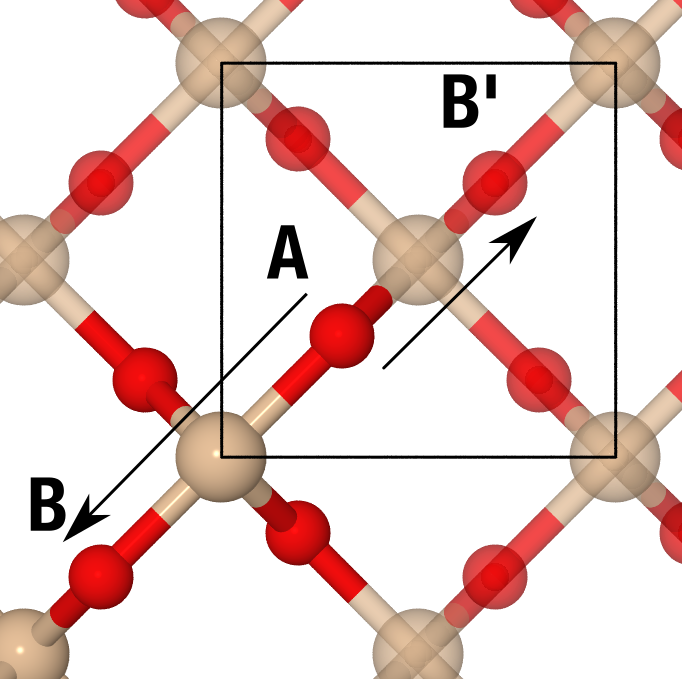
\includegraphics[width=0.25\textwidth]{img/micM_1.png}
    \caption{Vista desde el vector de celda $\mathbf{c}$ del SiO$_2$ tetragonal. Las esferas en color sólido pertenecen a la celda mostrada, mientras que las transparentes pertenecen a celdas vecinas.}
    \label{fig:mic1}
\end{figure}
\end{frame}

\begin{frame}{Algoritmo}
\begin{columns}
\begin{column}{0.6\textwidth}
	Procedimiento utilizado en el código para filtrar pares atómicos:
	\begin{enumerate}
		\item Evaluar distancia en la celda unitaria central (coordenadas relativas $(0,0,0)$.
		\item Evaluar distancia en las celdas circundantes ($(i,j,k)$, con $i,j,k = 0$ o $1$).
		\item Conservar la menor de las distancias obtenidas.
		\item Evaluar (\ref{cond}) y guardar la información del par si cumple la condición.
	\end{enumerate}
	\textit{Nota:} Solo se evalúan los traslapes $AB$, equivalentes a los traslapes $BA$, y los $AA$ se almacenan en automático.
\end{column}
\begin{column}{0.4\textwidth}
\begin{figure}
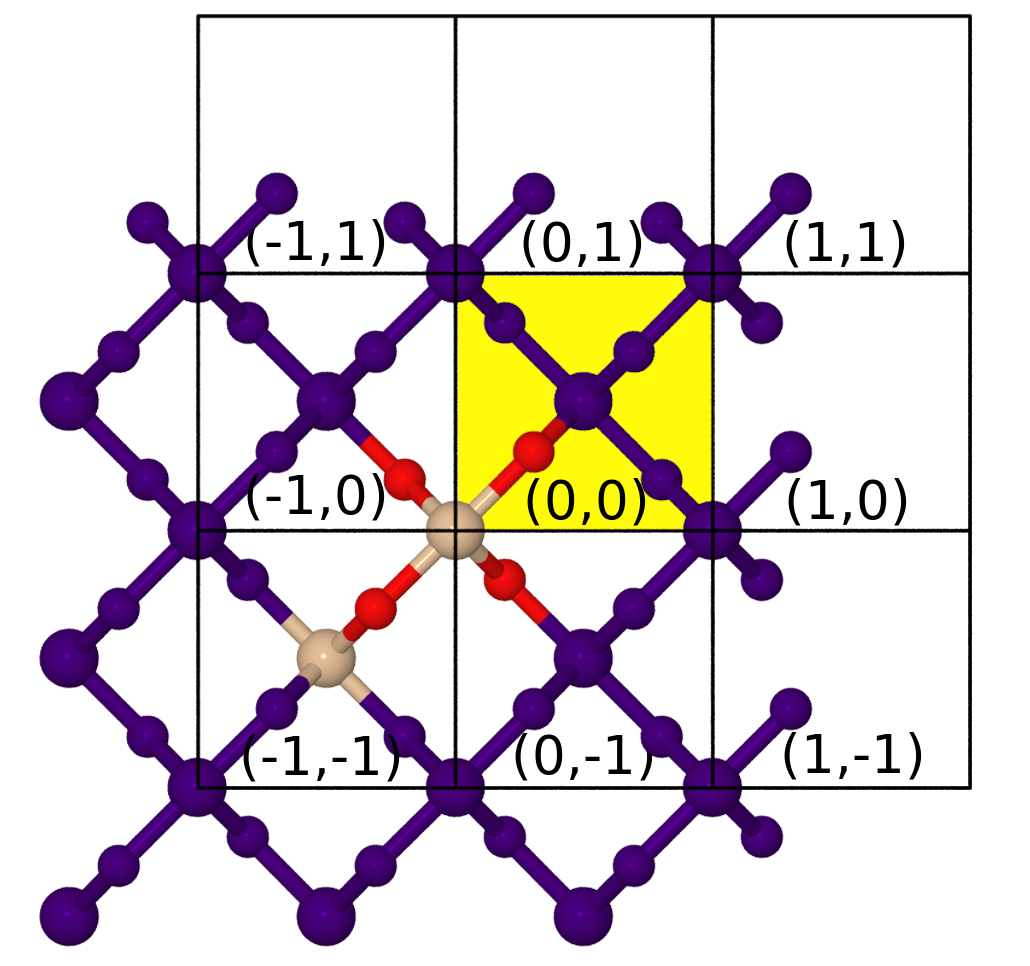
\includegraphics[width=0.9\textwidth]{img/surrCellSio2_4}
\caption{Celda $\mathbf{g_0}$ y sus átomos asignados, junto con las celdas circundantes y sus átomos (en morado). Hay 9 celdas circundantes arriba y 9 abajo del plano.}
\end{figure}
\end{column}
\end{columns}
\end{frame}

\begin{frame}
	Luego del filtrado de pares atómicos se procede al filtrado por capa.
	\begin{itemize}
		\item Se toma como referencia la lista de pares atómicos aceptados.
		\item Para capas en un mismo átomo (pares $AA$) solamente se evalúa (\ref{cond}) entre capas $\lambda_m$ y $\lambda_n$, dado que el caso $\lambda_n \lambda_m$ es equivalente y $\lambda_m$ $\lambda_m$ es igual a 1. 
		\item Si la comparación es entre capas de átomos $AB$ entonces $\lambda_m$ $\lambda_n$ y $\lambda_n$ $\lambda_m$ deben ser evaluados. 
		\item Se obtiene una lista de pares de capas con la información del par atómico y de las gaussianas primitivas correspondientes.
	\end{itemize}
\end{frame}

\begin{frame}{Producción de puntos de la malla}
Los puntos de la malla de un sistema periódico tridimensional cumplen con:
\begin{equation}
    \mathbf{g} = n_a \mathbf{a} + n_b \mathbf{b} + n_c \mathbf{c},
\end{equation}
con $\mathbf{a,b,c}$ los vectores base y $n_a,n_b,n_c$ coeficientes enteros. 

Las contribuciones coulómbica ($C_{\mu \nu}^\mathbf{g}$) y de intercambio ($X_{\mu \nu}^\mathbf{g}$) a la matriz de Fock contienen sumas sobre puntos de la malla (vectores $\mathbf{g,g'}$ y $\mathbf{h}$)(cantidad infinita):

\begin{equation}\label{C12}
C_{\mu \nu}^\mathbf{g} =\sum_{\sigma , \omega} \sum_{\mathbf{g'}} P_{\sigma \omega}^{\mathbf{g'}} \sum_\mathbf{h}  <\chi_\mu^\mathbf{0} \chi_\nu^\mathbf{g}|\frac{1}{|\mathbf{r_1-r_2}|}|\chi_\sigma^\mathbf{h} \chi_\omega^{\mathbf{h+g'}}> 
\end{equation}

\begin{equation}\label{X12}
X_{\mu \nu}^\mathbf{g} =-\frac{1}{2} \sum_{\sigma , \omega} \sum_{\mathbf{g'}} P_{\sigma \omega}^{\mathbf{g'}} \sum_\mathbf{h}  <\chi_\mu^\mathbf{0} \chi_\sigma^\mathbf{h}|\frac{1}{|\mathbf{r_1-r_2}|}|\chi_\nu^\mathbf{g} \chi_\omega^{\mathbf{h+g'}}>
\end{equation}

\end{frame}

\begin{frame}
Es necesario construir un subconjunto de la malla ($G$) a evaluar.

Los puntos en $G$ deben:
\begin{itemize}
	\item Estar alrededor del origen de la celda unitaria central ($\mathbf{g_0}$).
	\item Ser tales que al evaluar el traslape entre una GA alrededor de $\mathbf{g_0}$ y otra fuera de $G$ el traslape no cumplirá cierto criterio de tolerancia.
\end{itemize} 
\end{frame}

\begin{frame}{Algoritmo}
\begin{block}{Procedimiento utilizado}
Incluir en $G$ los puntos dentro de un cubo circunscrito por una esfera de radio $r_{cut}$. Usaremos la convención de alinear $\mathbf{a}$ con el eje $x$, que $\mathbf{b}$ se encuentre en el plano $xy$, y que $\mathbf{c}$ tenga componente $z$ positiva. 
\end{block}
\begin{columns}
\begin{column}{0.6\textwidth}
\begin{itemize}
\item Se calcula el valor fraccionario de $na, nb$ y $nc$ necesarios para alcanzar $r_{cut}$ sobre $x$, $y$ y $z$, respectivamente, aumentando un índice a la vez (variables $n_a^{lim}, n_b^{lim}$ y $n_c^{lim}$)
\item Se calcula la fracción que representan las componentes $b_x$ y $c_x$ respecto de $a_x$, así como la fracción que representa $c_y$ de $b_y$ (variables $n_b^{xf}, n_c^{xf}$ y $n_c^{yf}$).
\end{itemize} 
\end{column}
\begin{column}{0.39\textwidth}
\begin{figure}
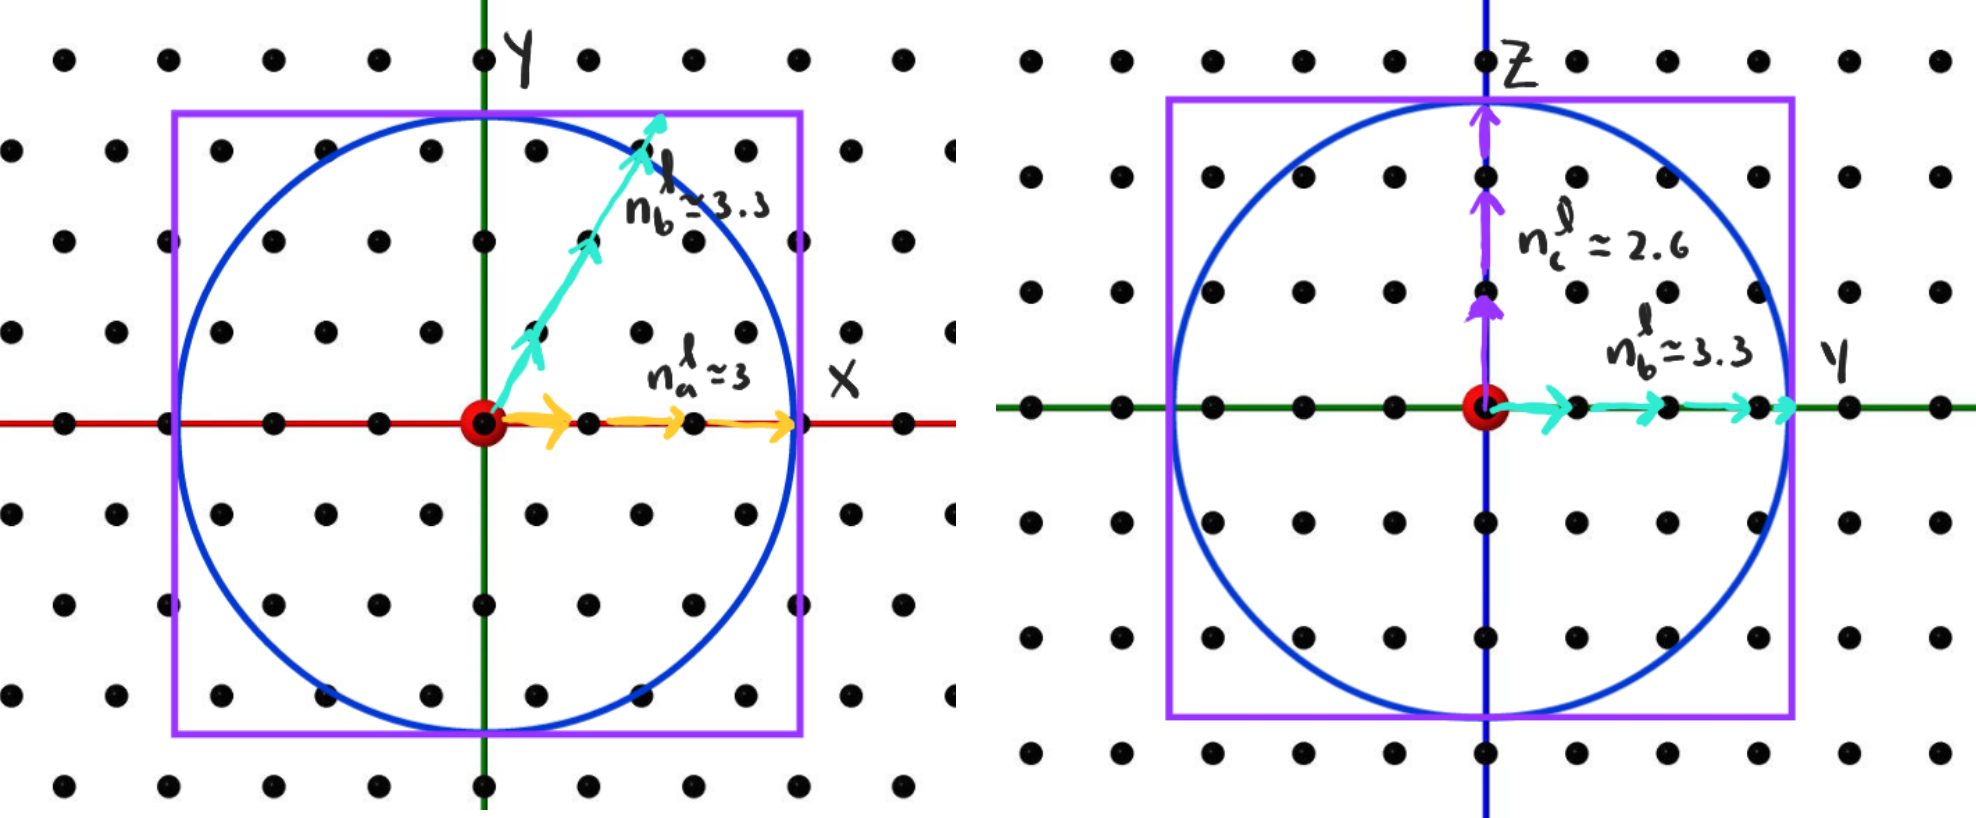
\includegraphics[width=0.9\textwidth]{img/Grid1_1}
\end{figure}
\vspace{-0.5cm}
\begin{figure}
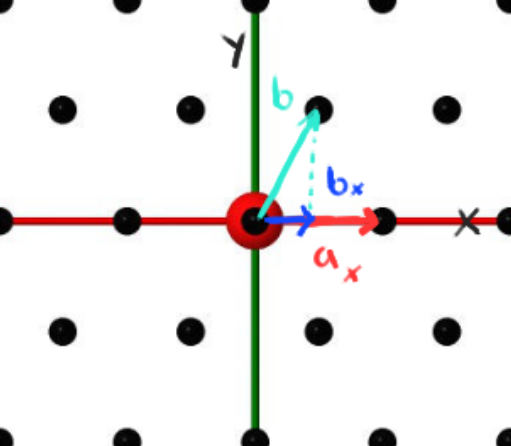
\includegraphics[width=0.5\textwidth]{img/gridProj}
\end{figure}
\end{column}
\end{columns}

\end{frame}

\begin{frame} 
\begin{itemize}
\item \textbf{Ciclo 1}: sobre el valor de $n_c$, del \textit{suelo} de $-n_c^{lim}$ (entero menor y más cercano a $-n_c^{lim}$) al \textit{techo} de $n_c^{lim}$ (entero mayor y más cercano a $n_c^{lim}$), con incrementos unitarios. 
\begin{itemize}
\item Solo $\mathbf{c}$ tiene componente sobre $z$. En este ciclo se determinan los valores de $n_c$ para cualquier punto.
\item Dentro calculamos una corrección sobre $n_b$ determinada por $n_c^{yf}$ y el valor actual de $n_c$ (variable $n_b^{corr}$).
\end{itemize}
\item \textbf{Ciclo 2}: dentro del Ciclo 1, va sobre $n_b$. Comienza en el suelo de $-n_b^{lim}-n_b^{corr}$ y termina en el techo de $n_b^{lim}-n_b^{corr}$, con incrementos unitarios. 
\begin{itemize}
\item Al considerarse $n_b^{corr}$ dado $n_c$ para la coordenada correspondiente en $z$ nos aseguramos de incluir los puntos dentro del cubo en la dirección $y$.
\item Dentro se realiza una corrección $n_a^{corr}$ obtenida usando $n_b^{xf}$, $n_c^{xf}$, y el valor actual de $n_b$ y $n_c$.
\end{itemize}
\end{itemize}
\end{frame}

\begin{frame}
\begin{columns}
\begin{column}{0.6\textwidth}
\begin{itemize}
\item \textbf{Ciclo 3}: dentro del Ciclo 2, sobre $n_a$. Comienza en el suelo de $-n_a^{lim}-n_a^{corr}$ y termina en el techo de $n_a^{lim}-n_a^{corr}$, con incrementos unitarios.
\begin{itemize}
\item Dentro utilizamos una función que añade un punto $(n_a,n_b,n_c)$ al arreglo $G$ dentro del objeto \textit{Preclas}.
\end{itemize}
\end{itemize}

\textit{Nota:} En realidad, incluimos una hilera adicional de puntos en $x,y,z$ a los contenido dentro del cubo.
%\begin{figure}
%    \centering
%    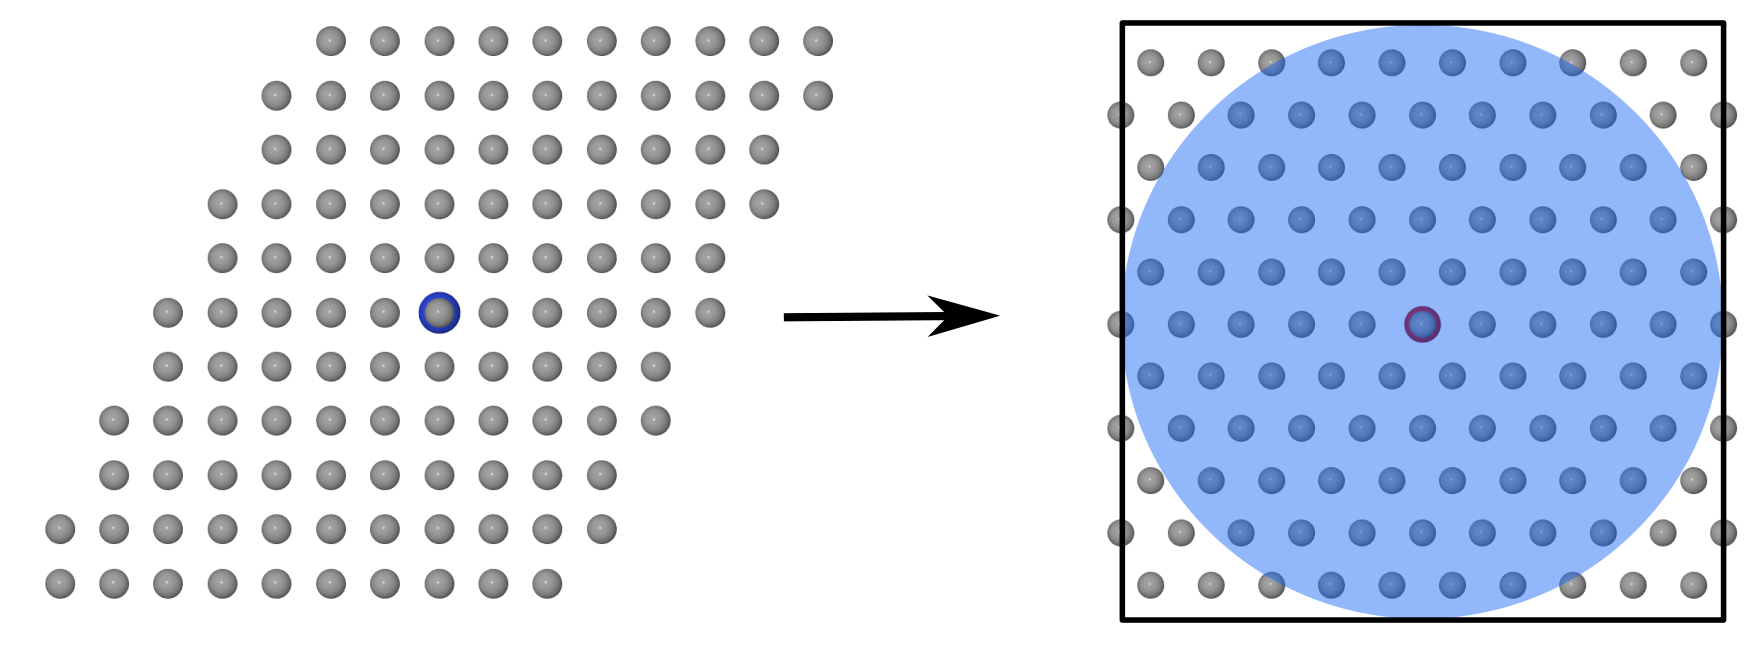
\includegraphics[width=0.6\textwidth]{img/gridGen.png}
%    \caption{A la izquierda, puntos generados de la malla para cuarzo-$\alpha$ en coordenadas relativas. A la derecha, estos puntos en espacio real. Se muestra el cubo que contiene dichos puntos, circunscrito a la esfera de radio $r_{cut}$.}
%    \label{fig:gridGen}
%\end{figure}
\end{column}
\begin{column}{0.35\textwidth}
\begin{figure}
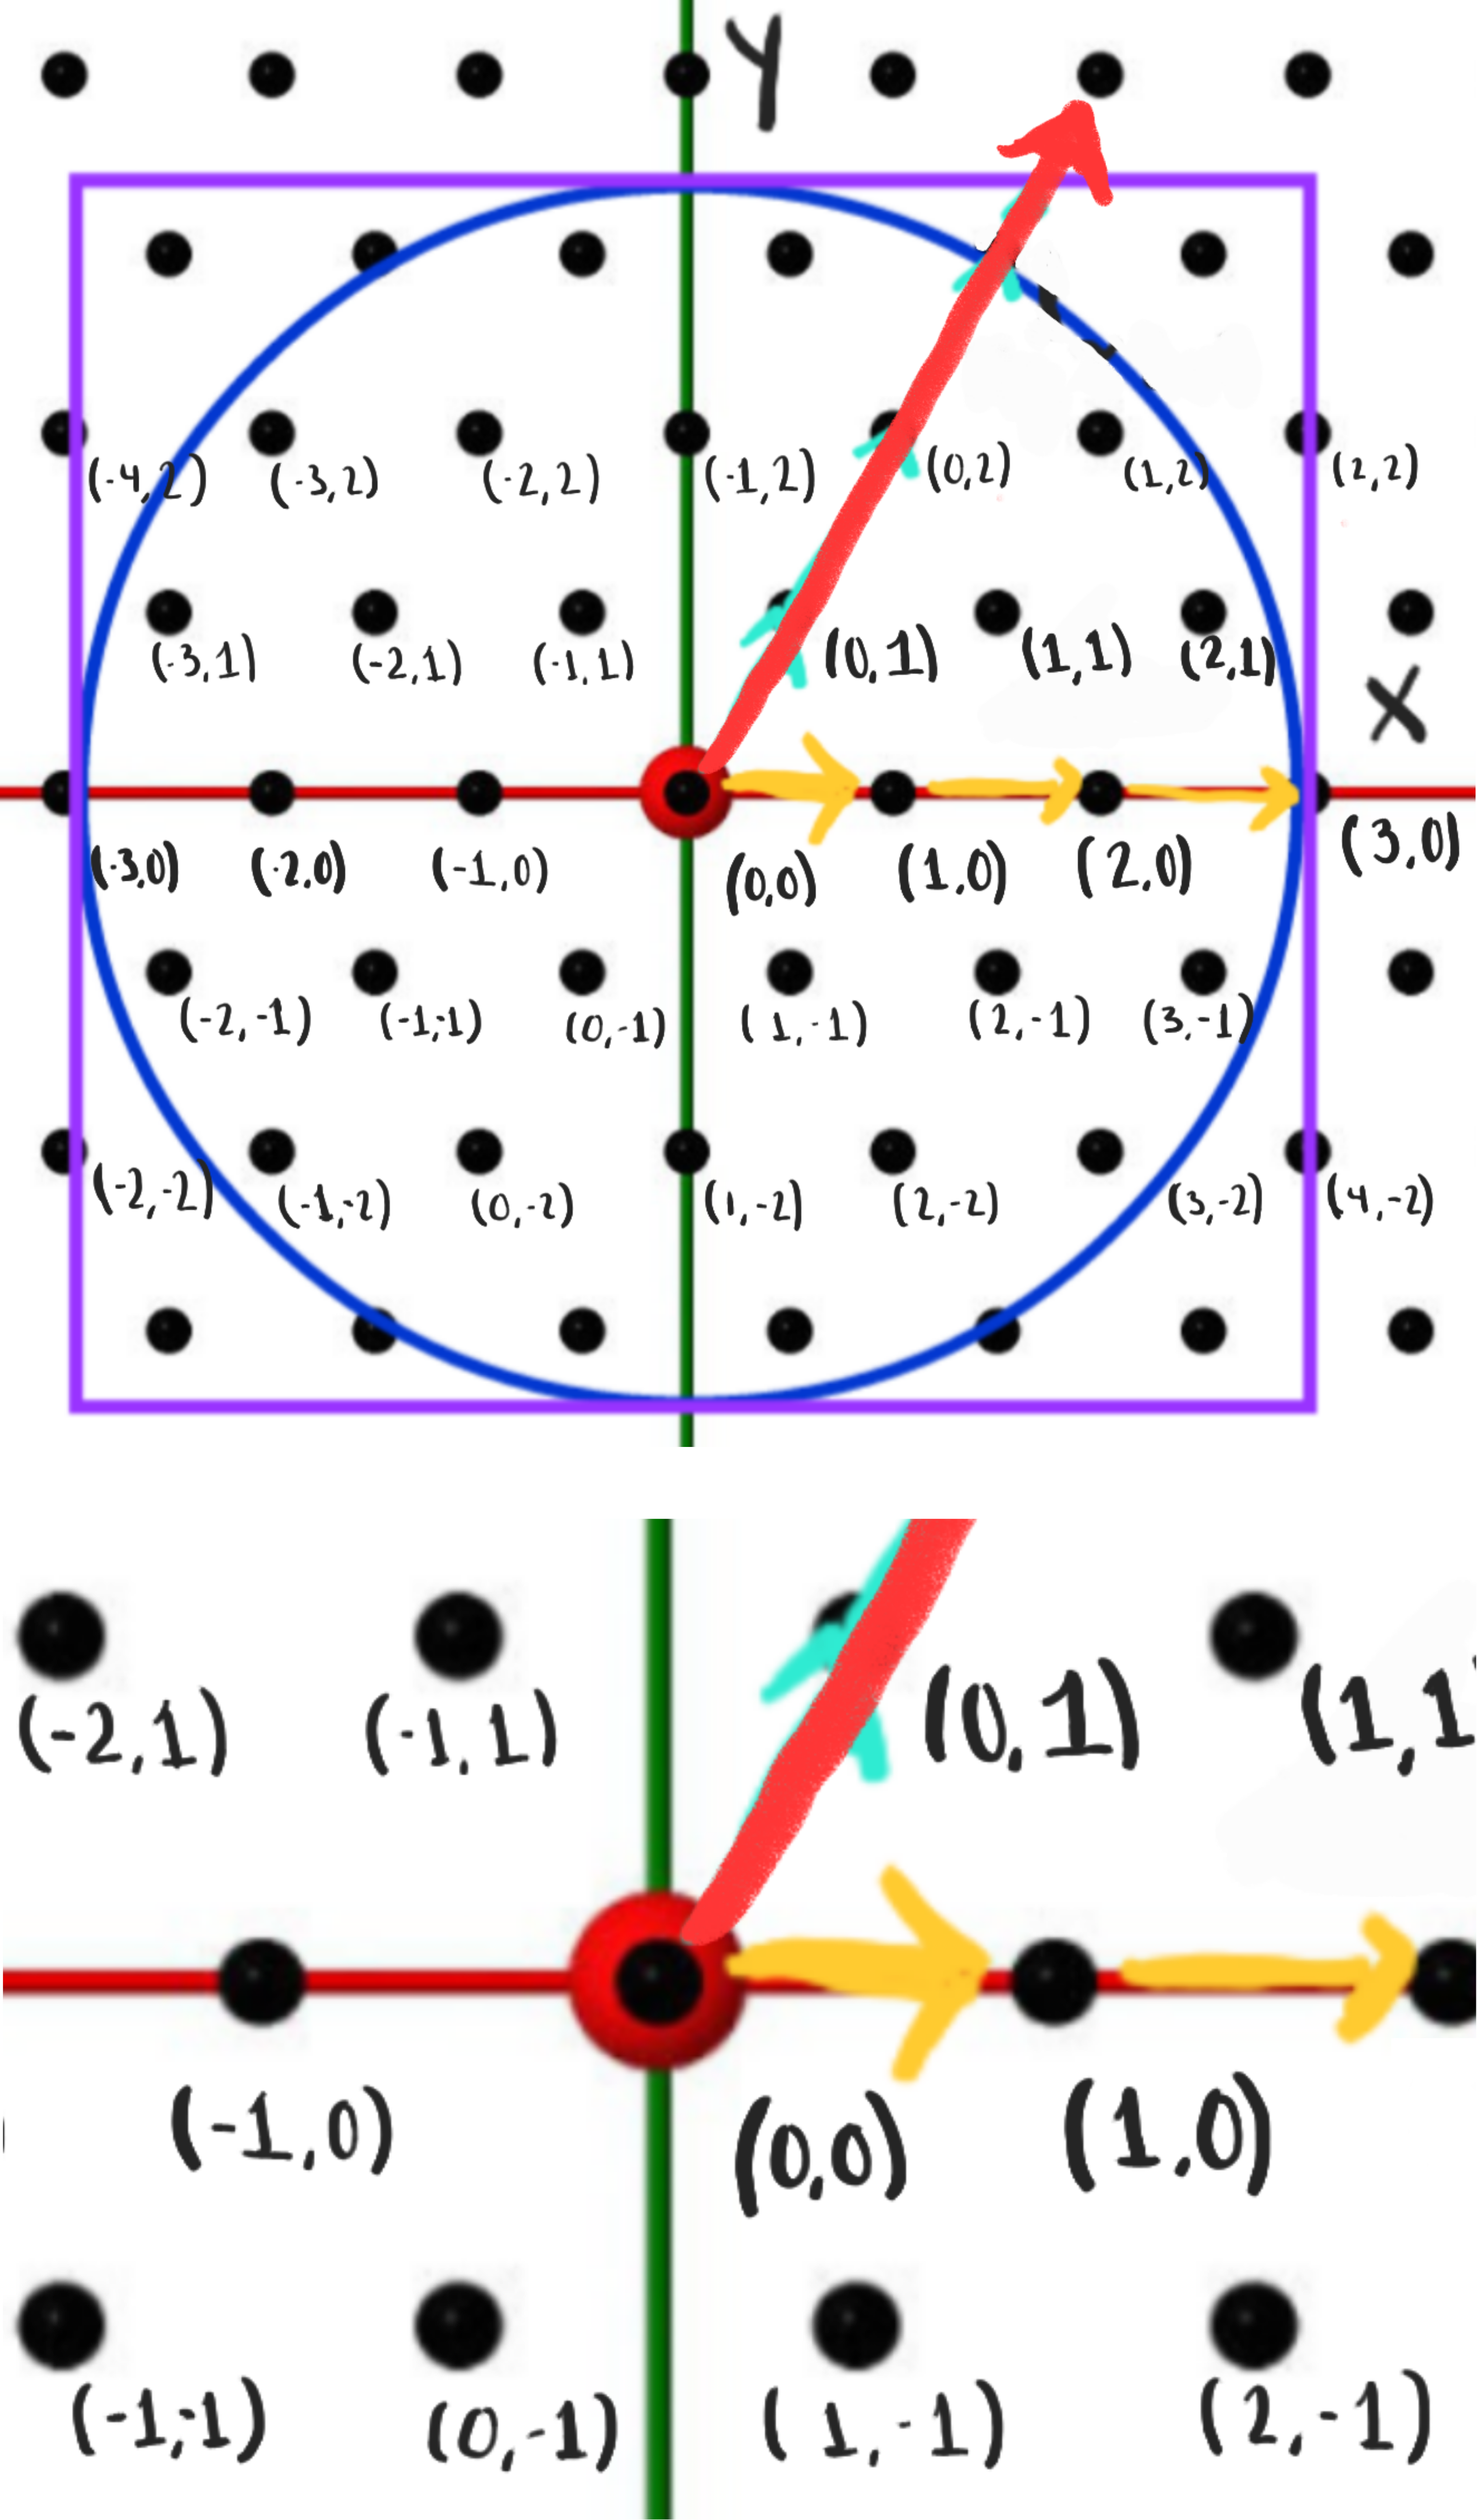
\includegraphics[width=0.9\textwidth]{img/gridPoint}
\end{figure}
\end{column}
\end{columns}
\end{frame}

\begin{frame}
\begin{figure}
\animategraphics[width=0.4\textwidth,controls,loop]{10}{gridSio2Small/gridSio2Z00}{001}{227}
\animategraphics[width=0.4\textwidth,controls,loop]{40}{gridSio2XSmall/gridSio2X00}{001}{227}
\caption{Producción de $G$ para cuarzo-$\alpha$ desde $z$ (izq) y desde $x$ (der).}
\end{figure}
\end{frame}

\section{Trabajo en progreso}
\begin{frame}{Matriz de traslape}
Un elemento de la matriz de traslape $\bm{\mathcal{S}}$ etiquetada por $\mathbf{g}$ cumple la siguiente expresión:

\begin{equation}
\mathcal{S}^\mathbf{g}_{\mu\nu} = <\chi_\mu|\chi_\nu^\mathbf{g}>    
\end{equation}

Con las listas obtenidas del filtrado de pares atómico de capas, y con la lista de puntos de la malla, podemos construir la mitad inferior de cada matriz $\bm{\mathcal{S}}^{\mathbf{g}}$. 

Esta información pude ser empatada con la obtenida por el programa Crystal, que cuenta con una opción para imprimir secciones de $\bm{\mathcal{S}}$. 

\end{frame}

\begin{frame}
En Crystal los orbitales atómicos $\chi_\mu$ están formados de la siguiente manera:

\begin{equation}\label{aoInRSG}
\chi_{\mu}(\mathbf{r-R_A-g}) = N_\lambda \sum_j d_j^\lambda G_{\ell}^m (\alpha_j^\lambda;\mathbf{r-R_A-g}),
\end{equation}
con $d_j$ y $\alpha_j$ son los coeficientes y exponentes fijos de la capa $\lambda$ a la que pertenece $\chi$, y $N_\lambda$ la constante de normalización de $\chi$. $G_{\ell}^m$ son funciones tipo gaussianas, las cuales en Crystal son Gaussianas Armónicas Reales (GAR):

\begin{equation}
G_{\ell}^m (\alpha_j^\lambda;\mathbf{r-R_A-g}) = c_j^{\ell,m} X_\ell^m(\mathbf{r}) e^{-\alpha_j^\lambda r^2},
\end{equation}

con $c_j^{\ell,m}$ la constante de normalización de $G_{\ell}^m$ y $X_\ell^m$ un armónico esférico real. 

\end{frame}

\begin{frame}{En proceso}
\begin{itemize}
\item Para $N_\lambda$ y $c_j^{\ell,m}$ se conocen expresiones para cualquier valor de $\ell$ y $m$ ($N_\lambda$ solo depende de los coeficientes y exponentes de $\lambda$). Estas están siendo programadas para $\ell=0,1,2$.
\item Al final tendremos la integral de un producto de GARs. En Crystal se sigue el esquema propuesto por Saunders basado en el de McMurchie-Davidson (S-MD), donde se expande el producto de dos GARs en Gaussianas Tipo Hermite.
\item Hay que implementar la solución de la integral de traslape en el esquema S-MD.
\end{itemize}
\end{frame}

\begin{frame}

\begin{block}{Notas}
\begin{itemize}
\item Las bibliotecas (y la mayoría de las metodologías) de las que se tiene conocimiento para la evaluación de IBs utilizan Gaussianas Cartesianas (GC). Con fines de validación se busca implementar esta metodología usando GARs para evaluar $\bm{\mathcal{S}}$, pero las IBs serán evaluadas utilizando GCs para poder usar la biblioteca externa.
\item La cantidad de integrales a evaluar aquí puede comenzar a ser considerable, por lo que se implementaran instrucciones de OpenACC para comenzar a probar los efectos del uso de GPUs en la evaluación de las integrales.
\end{itemize}
\end{block}
\end{frame} 

\begin{frame}{Perspectivas actuales}
Desarrollar la clase \textit{CryBiInfo}:

\begin{itemize}
    \item Filtrado de vectores de la malla dadas las tolerancias $T_1$, $T_2$, $T_3$, $T_4$ y $T_5$.
    \item Cálculo del tamaño de las matrices a construir.
    \item Cálculo de cantidades requeridas según el esquema a utilizar para la resolución de las integrales bielectrónicas.
\end{itemize}

Con la información de CryBiInfo podrán crearse \textit{CryCol} y \textit{CryEx}, dentro de los cuales se busca evaluar y almacenar las integrales bielectrónicas. $^a$

Cálculos en proceso:
\begin{itemize}
\item Estudio de CaTiO$_3$ con una vacancia de Oxígeno.
\item Efecto de $x$ en el Band Gap de SnZr$_{1-x}$Ti$_x$O$_3$.
\end{itemize}

\end{frame}

\setbeamertemplate{background}{\tikz[overlay,remember picture]\node[opacity=0.8]at (11.5,-6){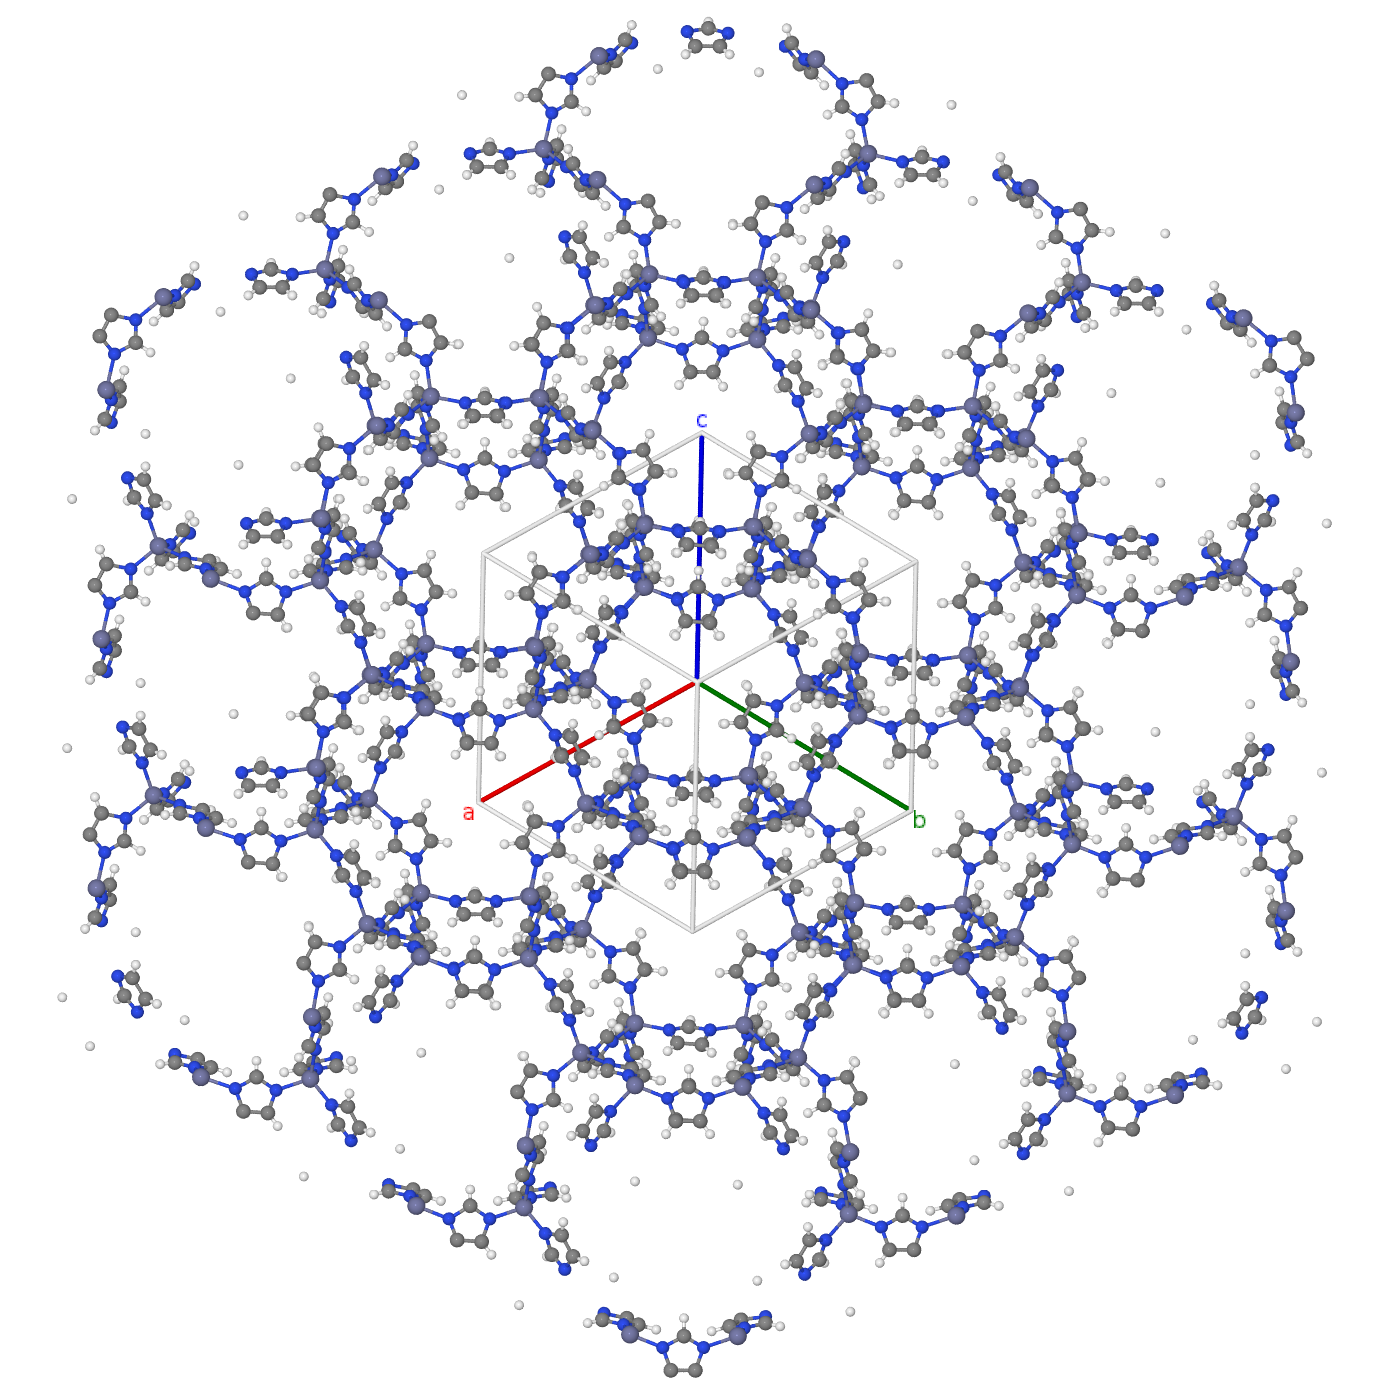
\includegraphics[width=10cm]{img/zif8}};
\tikz[overlay,remember picture]\node[opacity=0.8]at (3.7,-7){
\includegraphics[width=4.5cm]{img/uaml}};
\tikz[overlay,remember picture]\node[opacity=0.8]at (4,-1.5){
\includegraphics[width=7.5cm]{img/logodep}};}
\begin{frame}[standout]
\begin{flushleft}
{\Large Gracias por su atención.}
\end{flushleft}
\end{frame}

\appendix
%\setbeamertemplate{headline}{}
%\addtobeamertemplate{frametitle}{\vspace*{-\headheight}}{}
%\setbeamercolor{section in head/foot}{fg=normal text.bg, bg=structure.fg}
%
%\begin{frame}
%
%Experiencia personal: óxidos de metales de transición (colaboración con Dr. Federico González).
%\begin{block}{Efecto de distintas proporciones en SrZr$_x$Ti$_{1-x}$O$_3$.}
%\begin{itemize}
%%\item PBE0, 12x12x12 puntos $k$
%\item Para $x=1,0$ (grupo $Pm\overline{3}m$), con 40 procesadores, 40-85 minutos para optimizar geometría.
%\item Para $x=0.125$, $0.25$ y $0.5$, es necesario usar una supercelda y disminuir la simetría. Con 64 procesadores, 5,879-18,206 minutos (19,579 horas/CPU en el último). Por cada $x$ hay distintas distribuciones. {\firamedium 270,819 horas/CPU} de \textit{medio} proyecto (sin contar cálculos fallidos).
%%\item Sr$_{0.9955}$Pr_$_{0.003}$Zr$_x$Ti$_{1-x}$O$_3$.
%\end{itemize}
%\end{block}
%\begin{block}{Defectos en CaTiO$_3$}
%\begin{itemize}
%\item Pruebas sobre vacancia de oxígeno, con supercelda para lograr una proporción de 0.021\% del O en la celda.
%\item {\firamedium 72,128 horas/CPU} optimización. 
%\end{itemize}
%\end{block}
%\end{frame}
%
%\begin{frame}{Integrales bielectrónicas en sistemas finitos}
%
%En HF o KS-DFT, las contribuciones Coulómbica y de Intercambio (exacto) tienen la forma:
%
%\begin{equation}\label{ECoF}
%E_{J}=\frac{1}{2} \sum_{\mu \nu} P_{\mu \nu} \sum_{\sigma \omega} P_{\sigma \omega}  <\chi_\mu \chi_\nu | \chi_\sigma \chi_\omega> , 
%\end{equation}
%\begin{equation}\label{EExF}
%E_{X}=-\frac{1}{4} \sum_{\mu \nu} P_{\mu \nu} \sum_{\sigma \omega} P_{\sigma \omega}  <\chi_\mu \chi_\sigma | \chi_\nu \chi_\omega>	,
%\end{equation}
%
%donde $P_{\mu\nu} = 2 \sum_a c_{\mu a} c_{\nu a}^*$ es un elemento de la matriz densidad. Las cuatro sumas van sobre todos los orbitales atómicos $\chi$.
%
%
%Encontramos las \textbf{IB}: \colorbox{light-gray}{$\displaystyle <\mu \nu | \sigma \omega> = \int \int d\mathbf{r_1} d\mathbf{r_2} \chi_\mu \chi_\nu \frac{1}{|\mathbf{r_1-r_2}|} \chi_{\sigma} \chi_\omega$}
%
%
%\end{frame}
%
%\begin{frame}{Integrales bielectrónicas en sistemas periódicos}
%Nuestro potencial externo será periódico. Los orbitales deberán cumplir con el teorema de Bloch:
%%Los orbitales en la ecuación (\ref{monohf}) deberán cumplir con el teorema de Bloch:
%
%\begin{equation}\label{bloch}
%\psi(\mathbf{r} + \mathbf{g}) = e ^{i\mathbf{k \cdot g}} \psi(\mathbf{r}),
%\end{equation}
%$\mathbf{g}$ un vector de la malla directa, y $\mathbf{k}$ un vector en espacio recíproco.
%
%
%Varias formas de escribir orbitales que cumplan (\ref{bloch}). Nos interesa la técnica de combinación lineal de funciones localizadas. Nuestros orbitales \textit{cristalinos} serán:
%
%\begin{equation}
%\psi_\mathbf{n} (\mathbf{r; k}) =  \sum_\mu c_{\mu, \mathbf{k}}^\alpha \Phi_{\mu, \mathbf{k}} (\mathbf{r - R_\alpha}),
%\end{equation}
%
%\end{frame}
%
%\begin{frame}
%$\Phi$ es una \textit{función de Bloch}:
%%\frac{1}{\sqrt{N}}
%\begin{equation}
%\Phi_{\mu , \mathbf{k}} (\mathbf{r}) =  \sum_\mathbf{g} e ^{i\mathbf{k \cdot g}} \chi_\mu (\mathbf{r - R_\mu - g}),
%\end{equation}
%donde la suma sobre $\mathbf{g}$ va sobre todos los vectores de la malla.
%
%De nuevo podemos escribir nuestras ecuaciones en términos de la base de orbitales atómicos.
%
%\end{frame}
%
%\begin{frame}
%\begin{block}{Energía coulómbica y de intercambio de una celda del cristal}
%
%\begin{equation}\label{ECo}
%E_{J}=\frac{1}{2} \sum_{\mu \nu} \sum_\mathbf{g} P^\mathbf{g}_{\mu \nu} \sum_{\sigma \omega} \sum_\mathbf{g'} P^\mathbf{g'}_{\sigma \omega} \sum_\mathbf{h} <\underbrace{\chi_\mu^\mathbf{0} \chi_\nu^\mathbf{g}}_{T_1}\overbrace{|\frac{1}{|\mathbf{r_1-r_2}|}|\underbrace{\chi_\sigma^\mathbf{h} \chi_\omega^\mathbf{h+g'}}_{T_1}}^{T_2}> 
%\end{equation}
%\begin{equation}\label{EEx}
%E_{X}=-\frac{1}{4} \sum_{\mu \nu} \sum_\mathbf{g} \underbrace{P^\mathbf{g}_{\mu \nu}}_{T_4} \sum_{\sigma \omega} \sum_\mathbf{g'} \underbrace{P^\mathbf{g'}_{\sigma \omega}}_{T_5} \sum_\mathbf{h} <\underbrace{\chi_\mu^\mathbf{0} \chi_\sigma^\mathbf{h}}_{T_3}|\frac{1}{|\mathbf{r_1-r_2}|}|\underbrace{\chi_\nu^\mathbf{g} \chi_\omega^\mathbf{h+g'}}_{T_3}> 
%\end{equation}
%
%\end{block}
%
%\begin{itemize}
%%\item Por la invarianza translacional, podemos siempre ubicar en la celda de origen uno de los orbitales. Solo hay 3 sumas sobre vectores de malla.
%\item Las sumas son infinitas. Pueden acotarse usando criterios de truncamiento. En Crystal, hay 5 tolerancias asociadas al traslape entre pares de gaussianas.
%\end{itemize}
%
%\end{frame}
%
%\begin{frame}{Tolerancias}
%Si el traslape es menor a $10^{-T_i}$, se truncan o aproximan las sumas infinitas.
%\begin{table}[h]
%\begin{tabular}{|c |p{2.5cm}| p{6cm}|}
%\hline
%\rowcolor{blue!75}
%{\color{white}$T_i$} &\textcolor{white}{Sumas} &\textcolor{white}{Traslape}\\
%\hline
%\rowcolor{blue!20}
%$T_1$ & $\sum_\mathbf{g}$ o $\sum_\mathbf{g'}$ en $J$ & GAs de $<\mu^{\mathbf{0}}|\nu^{\mathbf{g}}>$ o $<\sigma^{\mathbf{h}}|\omega^{\mathbf{h+g'}}>$\\
%$T_3$ & $\sum_\mathbf{h}$ en $X$ & GAs de $<\mu^\mathbf{0}|\sigma^\mathbf{h}>$ o $<\nu^\mathbf{g}|\omega^\mathbf{h+g'}>$\\
%\rowcolor{blue!20}
%$T_4$,$T_5$ & $\sum_\mathbf{g}$ , $\sum_\mathbf{g'}$ en $X$ & GAs de $<\mu^\mathbf{0}|\nu^\mathbf{g}>$ , $<\sigma^\mathbf{h}|\omega^\mathbf{h+g'}>$ \\
%$T_2$ & ${\color{red}\sum_\mathbf{h}}$ en $J$  &entre $\mu\nu$ y la GA de la capa de $\sigma^{\mathbf{h}}$\\
%\hline
%\end{tabular}
%
%\end{table}
%\begin{equation}
%E_{J}=\frac{1}{2} \sum_{\mu \nu} \sum_\mathbf{g} P^\mathbf{g}_{\mu \nu} \sum_{\sigma \omega} \sum_\mathbf{g'} P^\mathbf{g'}_{\sigma \omega} \sum_\mathbf{h} <\underbrace{\chi_\mu^\mathbf{0} \chi_\nu^\mathbf{g}}_{T_1}\overbrace{|\frac{1}{|\mathbf{r_1-r_2}|}|\underbrace{\chi_\sigma^\mathbf{h} \chi_\omega^\mathbf{h+g'}}_{T_1}}^{T_2}> 
%\end{equation}
%\begin{equation}
%E_{X}=-\frac{1}{4} \sum_{\mu \nu} \sum_\mathbf{g} \underbrace{P^\mathbf{g}_{\mu \nu}}_{T_4} \sum_{\sigma \omega} \sum_\mathbf{g'} \underbrace{P^\mathbf{g'}_{\sigma \omega}}_{T_5} \sum_\mathbf{h} <\underbrace{\chi_\mu^\mathbf{0} \chi_\sigma^\mathbf{h}}_{T_3}|\frac{1}{|\mathbf{r_1-r_2}|}|\underbrace{\chi_\nu^\mathbf{g} \chi_\omega^\mathbf{h+g'}}_{T_3}> 
%\end{equation}
%\end{frame}
%
%\begin{frame}{SC2020}
%Presentaciones interesantes del año:
%
%\begin{itemize}
%\item \textit{Pushing the Limit of Molecular Dynamics with Ab Initio Accuracy to 100 Million Atoms with Machine Learning}. En Summit (todo el equipo). 1 nanosegundo con 100 millones de átomos por día. 
%\item \textit{Scaling the Hartree-Fock Matrix Build on Summit}. The calculation ran for just over half an hour using 26,268 NVIDIA V100 Graphics Processing Units (GPUs) and simulated 20,063 water molecules at a resolution never before possible. 	
%\end{itemize}
%
%\end{frame}
%
%\begin{frame}
%\hspace*{-1cm}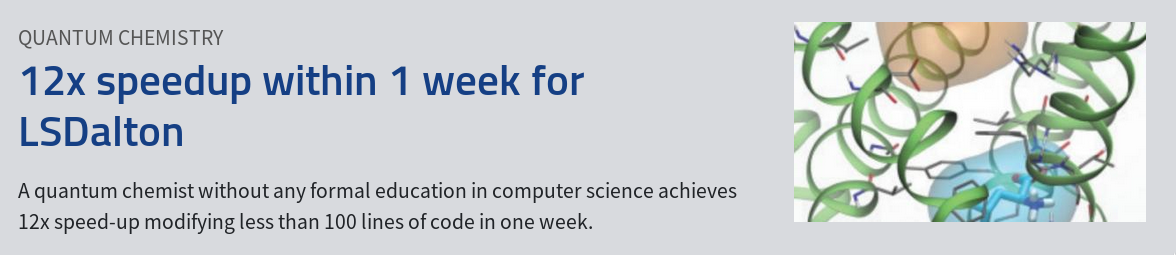
\includegraphics[width=15.9cm]{img/lsd1}\\
%\hspace*{-1cm}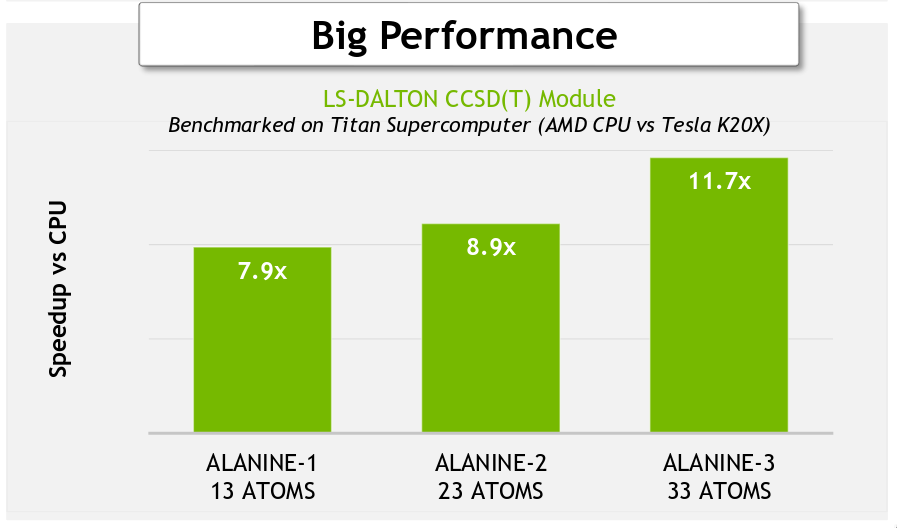
\includegraphics[width=8cm]{img/lsdg}
%\tikz [overlay]        
%        \node[text width=5cm,opacity=1] at
%        	(4cm,2.5cm) 
%        	{``(...)one of 13 application code projects to join the Center for Accelerated Application Readiness (CAAR) program. (...) among the first applications to run on Summit''};
%\end{frame}
%
%\begin{frame}
%
%\centering
%\hspace*{-1cm}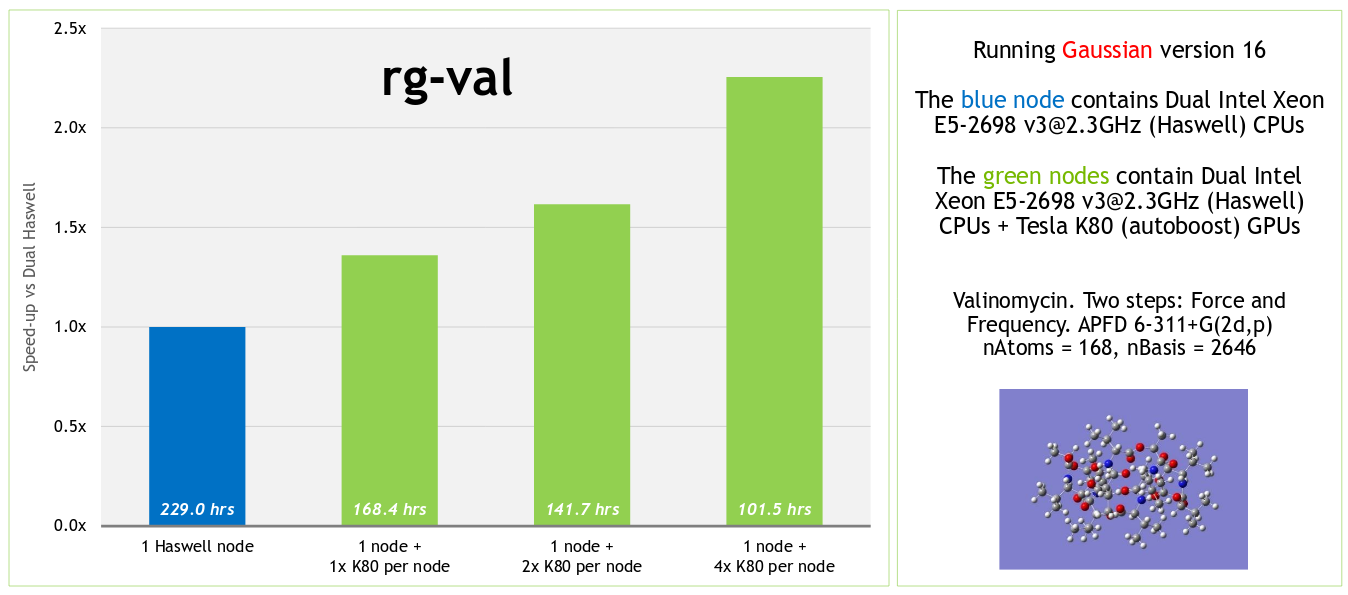
\includegraphics[width=15.8cm]{img/g16}
%\end{frame}
%\begin{frame}
%\centering
%\hspace*{-1cm}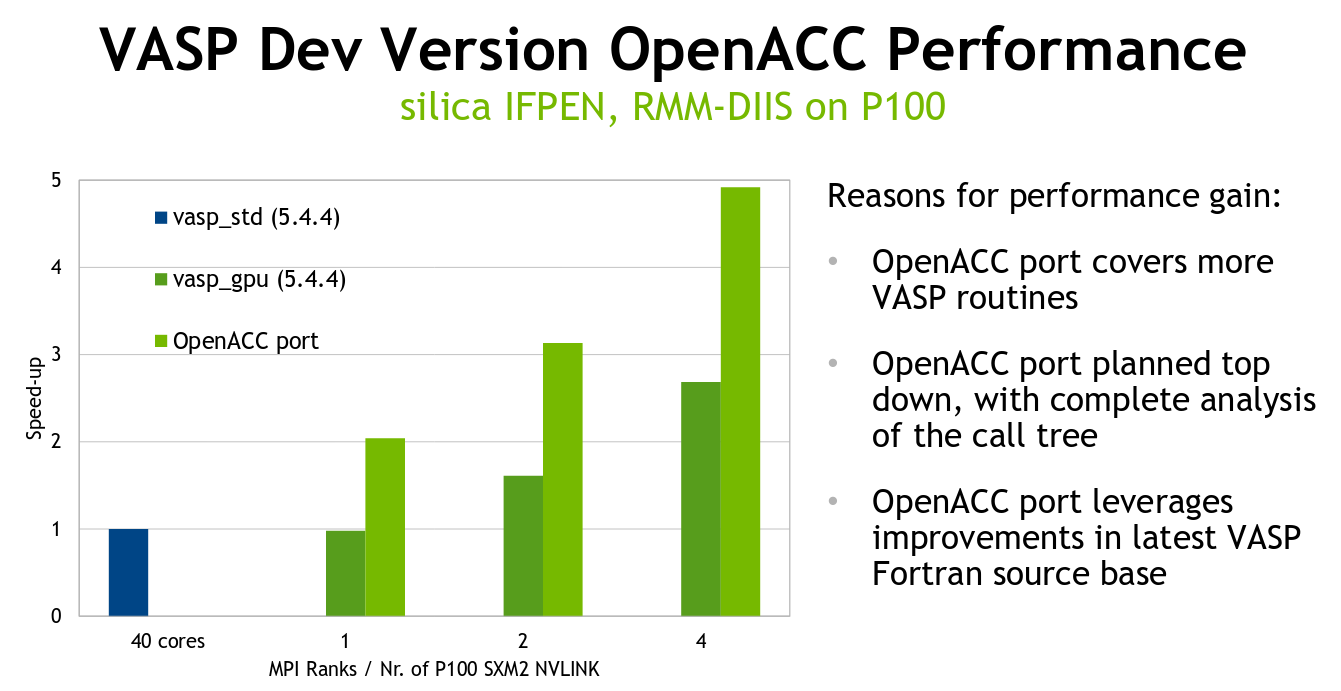
\includegraphics[width=15.8cm]{img/vasp}
%\end{frame}
%
%\begin{frame}{Malla periódica}
%    \begin{itemize}
%    \item La malla puede representarse en el espacio directo o en el espacio recíproco.
%    \end{itemize}
%    \begin{figure}[h]
%	\centering
%%	\hspace{-1.5cm}
%	\begin{subfigure}[c]{0.45\textwidth}
%	  \begin{tikzpicture}[scale=0.80]
    \coordinate (Origin)   at (-7,-4);
    \coordinate (XAxisMin) at (-3,0);
    \coordinate (XAxisMax) at (3,0);
    \coordinate (YAxisMin) at (0,-3);
    \coordinate (YAxisMax) at (0,3);
%    \draw [thin, gray,-latex] (XAxisMin) -- (XAxisMax);% Draw x axis
%    \draw [thin, gray,-latex] (YAxisMin) -- (YAxisMax);% Draw y axis

    \clip (-7.7,-0.5) rectangle (0.5,4.5); % Clips the picture...
    %\pgftransformcm{1}{0.0}{0.0}{1}{\pgfpoint{0cm}{0cm}}
          % This is actually the transformation matrix entries that
          % gives the slanted unit vectors. You might check it on
           % MATLAB etc. . I got it by guessing.
    \coordinate (Bone) at (0,1);
    \coordinate (Btwo) at (2,-2);
    \draw[style=help lines,dashed] (-14,-14) grid[step=1cm] (14,14);
          % Draws a grid in the new coordinates.
          %\filldraw[fill=gray, fill opacity=0.3, draw=black] (0,0) rectangle (2,2);
              % Puts the shaded rectangle
    \foreach \x in {-7,...,7}{% Two indices running over each
      \foreach \y in {-4,-3,...,4}{% node on the grid we have drawn 
        \node[draw,circle,inner sep=2pt,fill] at (\x,\y) {};
            % Places a dot at those points
      }
    }
    \draw [ultra thick,-latex,red] (-7,3)
        -- +(0,1) node [above left] {$\mathbf{a_1}$};
    \draw [ultra thick,-latex,red] (-7,3)
        -- +(1,0) node [below right] {$\mathbf{a_2}$};
    \draw [ultra thick,-latex,blue] (-7,1)
        -- (-6,2) node [below right] {$\mathbf{g}$};
    \draw [ultra thick,-latex,blue] (-7,1)
        -- (-5,0) node [above right] {$\mathbf{g'}$};
	    
    \filldraw[fill=gray, fill opacity=0.3, draw=black] (-3,3)
        rectangle (-2,4);
    \filldraw[fill=gray, fill opacity=0.3, draw=black] (-3,1)
        -- (-2,1) -- (-1,2) -- (-2,2) -- cycle;
    %\draw [thin,-latex,red, fill=gray, fill opacity=0.3] (0,0)
        % -- ($2*(0,2)+(2,-2)$)
        % -- ($3*(0,2)+2*(2,-2)$) -- ($(0,2)+(2,-2)$) -- cycle;
  \end{tikzpicture}
  \caption{Espacio directo}
  %\caption{Malla cuadrada en el espacio directo. Los vectores $\mathbf{a_1}$ y $\mathbf{a_2}$ son unos de los posibles vectores base de la malla; los vectores $\mathbf{g}$, $\mathbf{g'}$ y $\mathbf{g'}$ son combinaciones lineales de éstos. Las zonas sombreadas son  celdas unitarias. }
  \label{malla1}
%	\end{subfigure}
%	\hfill
%	\begin{subfigure}[c]{0.45\textwidth}
%	  \begin{tikzpicture}[scale=0.80]
    \coordinate (Origin)   at (-7,-4);
    \coordinate (XAxisMin) at (-3,0);
    \coordinate (XAxisMax) at (3,0);
    \coordinate (YAxisMin) at (0,-3);
    \coordinate (YAxisMax) at (0,3);
%    \draw [thin, gray,-latex] (XAxisMin) -- (XAxisMax);% Draw x axis
%    \draw [thin, gray,-latex] (YAxisMin) -- (YAxisMax);% Draw y axis

    \clip (-7.7,-0.5) rectangle (0.5,4.5); % Clips the picture...
    %\pgftransformcm{1}{0.0}{0.0}{1}{\pgfpoint{0cm}{0cm}}
          % This is actually the transformation matrix entries that
          % gives the slanted unit vectors. You might check it on
           % MATLAB etc. . I got it by guessing.
    \coordinate (Bone) at (0,1);
    \coordinate (Btwo) at (2,-2);
    \draw[style=help lines,dashed] (-14,-14) grid[step=1cm] (14,14);
          % Draws a grid in the new coordinates.
          %\filldraw[fill=gray, fill opacity=0.3, draw=black] (0,0) rectangle (2,2);
              % Puts the shaded rectangle
    \foreach \x in {-7,...,7}{% Two indices running over each
      \foreach \y in {-4,-3,...,4}{% node on the grid we have drawn 
        \node[draw,circle,inner sep=2pt,fill] at (\x,\y) {};
            % Places a dot at those points
      }
    }
    \draw [ultra thick,-latex,brown] (-7,3)
        -- +(0,1) node [left] {$\mathbf{b_1}$};
    \draw [ultra thick,-latex,brown] (-7,3)
        -- +(1,0) node [below right] {$\mathbf{b_2}$};
    \draw [ultra thick,-latex,orange] (-7,1)
        -- (-6,2) node [below right] {$\mathbf{K}$};
    \draw [ultra thick,-latex,orange] (-7,1)
        -- (-5,0.5) node [above right] {\small{$\mathbf{k'}$}};
    \draw [ultra thick,-latex,orange] (-5,0.5)
        -- (-4,0.5) node [right] {\small{$\mathbf{k'}+\mathbf{b_2}$}};    
    \filldraw[fill=gray, fill opacity=0.3, draw=black] (-3,2)
        -- (-2,1) -- (-1,2) -- (-2,3) -- cycle;
    \filldraw[fill=gray, fill opacity=0.3, draw=black] (-2.5,1.5)
        rectangle (-1.5,2.5) ;
    \filldraw[fill=gray, fill opacity=0.3, draw=black] (-3,1.5)
        rectangle (-1,2.5) ;
	\filldraw[fill=gray, fill opacity=0.3, draw=black] (-2.5,1)
        rectangle (-1.5,3) ;
        
    %\draw [thin,-latex,red, fill=gray, fill opacity=0.3] (0,0)
        % -- ($2*(0,2)+(2,-2)$)
        % -- ($3*(0,2)+2*(2,-2)$) -- ($(0,2)+(2,-2)$) -- cycle;
  \end{tikzpicture}
  \caption{Espacio recíproco}
  %\caption{Malla cuadrada en el espacio recíproco. Los vectores $\mathbf{b_1}$ y $\mathbf{b_2}$ son vectores base, $\mathbf{K}$ es combinación lineales de estos, y $\mathbf{k}$ es un punto cualquiera en este espacio. Las zonas sombreadas representan las primeras tres zonas de Brillouin; la primer zona de Brillouin es la más oscura. }
  \label{malla2}	
%	\end{subfigure}
%	\caption{Malla cuadrada en distintos espacios.}
%	\end{figure}
%\end{frame}
% 
%\begin{frame}{Matriz Densidad: ejemplo de conversión a espacio \textit{k}}
%La matriz densidad en el espacio recíproco, $\mathbf{P}(\mathbf{k})$, 
%\begin{equation}\label{dens1}
%P_{\mu \nu}(\mathbf{k})=\sum^{N occ.}_n c^*_{\mu n}(\mathbf{k}) c_{\nu n}(\mathbf{k}),
%\end{equation}
%donde $n$ es el índice de los estados, y los $c_{j n}(\mathbf{k})$ son los coeficientes de la combinación lineal usada para formar OC con las FB.
%
%La matriz densidad en el espacio directo, $P_{\mu \nu}^\mathbf{g}$,
%\begin{equation}
%P^\mathbf{g}_{\mu \nu}=\sum_n \frac{1}{V_{BZ}}\int_{BZ} d \mathbf{k} e^{i\mathbf{k\cdot g}} c^*_{\mu n}(\mathbf{k}) c_{\nu n}(\mathbf{k}) \theta (E_F-E_n(\mathbf{k})),
%\end{equation}
%donde $V_{BZ}$ es el volumen de la primera zona de Brillouin, $E_F$ es la energía de Fermi, $E_n$ la energía del $n$-ésimo estado, y $\theta (E_F-E_n(\mathbf{k}))$ es la función de Heaviside. 
%\end{frame}
%
%%\begin{frame}{Cronograma}
%%\begin{figure}
%%    \centering
%%    \begin{ganttchart}[
%%    vgrid,
%%    expand chart=\textwidth
%%   ]{1}{8}
%%   \gantttitle{Trimestres}{8}\\
%%   \gantttitle{20-O}{1} \gantttitle{21-I}{1} \gantttitle{21-P}{1} \gantttitle{21-O}{1} \gantttitle{22-I}{1} \gantttitle{22-P}{1} \gantttitle{22-O}{1} \gantttitle{23-I}{1}\\
%%   \gantttitle{2021}{3} \gantttitle{2022}{3} \gantttitle{2023}{2} \\
%%   \ganttbar[bar/.append style={fill=red}]{Rutina de clasificación}{1}{2}\\
%%   \ganttbar[bar/.append style={fill=red}]{Acoplamiento a código central}{3}{3}\\
%%   \ganttbar[bar/.append style={fill=red}]{Rutinas GPU}{4}{5}\\
%%   \ganttbar[bar/.append style={fill=blue!60}]{Aportaciones a código central}{3}{5}\\
%%   \ganttbar[bar/.append style={fill=blue!60, dashed}]{Artículo de biblioteca - moléculas}{5}{6}\\
%%   \ganttbar[bar/.append style={fill=red}]{Pruebas de ejecución}{6}{6}\\
%%   \ganttbar[bar/.append style={fill=red,dashed}]{Artículo de biblioteca - sólidos}{6}{7}\\
%%   \ganttbar[bar/.append style={fill=red}]{Integración}{7}{8}\\
%%   \ganttbar[bar/.append style={fill=green}]{Escritura de tesis}{6}{8}
%%   %\\\ganttbar{Task 1}{1}{2} 
%%   %\\\ganttlinkedbar{Task 2}{3}{7} 
%%   %\ganttnewline\ganttmilestone{Milestone}{7} 
%%   %\ganttnewline\ganttbar{Final Task}{8}{12}\ganttlink{elem2}{elem3}\ganttlink{elem3}{elem4}
%%\end{ganttchart}
%%\includegraphics[width=10cm]{img/chrono}
%    %\caption{Diagrama de Gantt. La fecha final del diagrama es Julio del 2023. En rojo se destacan las tareas centrales, en azul las asociadas a la implementación para moléculas, y en verde la escritura de la tesis. Las líneas punteadas indican posibles artículos a publicar.}
%%    \label{fig:my_label}
%%\end{figure}
%%\end{frame}
% 
\end{document}
